\documentclass[9pt]{beamer}
\usepackage{amsmath, amssymb, amsthm, mathtools, graphicx, float, subfigure, booktabs, enumitem}
\usepackage{hyperref}
\urlstyle{same}
\usepackage{minted}
\usepackage{pifont}
\usepackage{xcolor}
\usepackage[utf8]{inputenc} % usually not needed (loaded by default)
\usepackage[T1]{fontenc}
\hypersetup{colorlinks=true,citecolor=blue}
\usepackage{tikz}
\usepackage{fontawesome}
\usepackage{libertine}
\usepackage[libertine]{newtxmath}
\usetikzlibrary{calc,shapes}
\usepackage[normalem]{ulem}
\setbeamertemplate{theorems}[numbered]
\usepackage[authoryear,round]{natbib}
% \usepackage[portuguese]{babel}
\usetheme[pageofpages=of,% String used between the current page and the
                         % total page count.
          bullet=circle,% Use circles instead of squares for bullets.
          titleline=true,% Show a line below the frame title.
          alternativetitlepage=true,% Use the fancy title page.
          %titlepagelogo=logo-fiocruz,% Logo for the first page.
          %watermark=watermark-poli
          to,% Watermark used in every page.
          %watermarkheight=100px,% Height of the watermark.
          %watermarkheightmult=4,% The watermark image is 4 times bigger
                                % than watermarkheight.
          ]{Torino}
\usecolortheme{freewilly}          
%%%% Box options
\newcommand{\tikzmark}[1]{\tikz[overlay,remember picture] \node (#1) {};}
%%%% Background settings          
% \setbeamercolor{normal text}{fg=white,bg=black!90}
% \setbeamercolor{structure}{fg=white}
% \setbeamercolor{alerted text}{fg=red!85!black}
% \setbeamercolor{item projected}{use=item,fg=black,bg=item.fg!95}
% \setbeamercolor*{palette primary}{use=structure,fg=structure.fg}
% \setbeamercolor*{palette secondary}{use=structure,fg=structure.fg!95!black}
% \setbeamercolor*{palette tertiary}{use=structure,fg=structure.fg!90!black}
% \setbeamercolor*{palette quaternary}{use=structure,fg=structure.fg!95!black,bg=black!80}
% \setbeamercolor{title}{fg=white}
% \setbeamercolor{frametitle}{bg=white}
% \setbeamercolor*{framesubtitle}{fg=white}
% \setbeamercolor*{block title}{parent=structure,bg=black!95}
% \setbeamercolor*{block body}{fg=black,bg=black!10}
% \setbeamercolor*{block title alerted}{parent=alerted text,bg=black!95}
% \setbeamercolor*{block title example}{parent=example text,bg=black!95}


%%%% Maths crap
\newtheorem{remark}{Remark}[]
\newtheorem{theo}{Theorem}[]
\newtheorem{exercise}{Exercise}[]
\newtheorem{defn}{Definition}[]
\newtheorem{question}{Question}[]
\newtheorem{idea}{Idea}[]
\newtheorem{property}{Property}[]
%%%% Itemize settings 
\setlist[itemize,1]{label=$\bullet$}
\setlist[itemize,2]{label=$\diamond$}

% \setbeamercolor{block title}{use=structure,fg=white,bg=structure.fg!75!black}
% \setbeamercolor{block body}{parent=normal text,use=block title,bg=block title.bg!10!bg}

\setbeamercolor{block title}{use=structure,fg=white,bg=black}
\setbeamercolor{block body}{parent=normal text,use=block title,fg=white,bg=gray}
\setbeamercolor{frametitle}{bg=black, fg=white}

%%%%%%%%%%%%%%%%%%%% Notation stuff
\newcommand{\indep}{\perp \!\!\! \perp} %% indepence
\newcommand{\pr}{\operatorname{Pr}} %% probability
\newcommand{\vr}{\operatorname{Var}} %% variance
\newcommand{\rs}{X_1, X_2, \ldots, X_n} %%  random sample
\newcommand{\irs}{X_1, X_2, \ldots} %% infinite random sample
\newcommand{\rsd}{x_1, x_2, \ldots, x_n} %%  random sample, realised
\newcommand{\Sm}{\bar{X}_n} %%  sample mean, random variable
\newcommand{\sm}{\bar{x}_n} %%  sample mean, realised
\newcommand{\Sv}{\bar{S}^2_n} %%  sample variance, random variable
\newcommand{\sv}{\bar{s}^2_n} %%  sample variance, realised
\newcommand{\bX}{\boldsymbol{X}} %%  random sample, contracted form (bold)
\newcommand{\bx}{\boldsymbol{x}} %%  random sample, realised, contracted form (bold)
\newcommand{\bT}{\boldsymbol{T}} %%  Statistic, vector form (bold)
\newcommand{\bt}{\boldsymbol{t}} %%  Statistic, realised, vector form (bold)
\newcommand{\mle}{\hat{\theta}_{\text{MLE}}}
\newcommand{\mb}{\hat{\theta}_{\text{B}}}
\newcommand{\map}{\hat{\theta}_{\text{MAP}}}
\newcommand{\be}{\operatorname{Be}} %% probability
\DeclareMathOperator*{\argmin}{arg\,min}
\DeclareMathOperator*{\argmax}{arg\,max}
\DeclareMathOperator\supp{supp}
\usepackage{url}
%%%% Hyperref stuff
\hypersetup{
  colorlinks = true, %Colours links instead of ugly boxes
  urlcolor   = cyan, %Colour for external hyperlinks
  linkcolor  = cyan, %Colour of internal links
  citecolor  = red %Colour of citations
}
%%%% To create without the 'Figure' prefix. Remove if you need'em
\usepackage{caption}
\captionsetup[figure]{labelformat=empty}
%%%%
\author{
\underline{Luiz Max de Carvalho}[lmax.fgv@gmail.com]\linebreak
}
\title{
\Huge Bayesian Statistics
}
\institute{
PhD-level course\\
School of Applied Mathematics (EMAp/FGV), Rio de Janeiro.
}
\date{\today}
\logo{
\includegraphics[scale=.15]{logo.jpg}}
\begin{document}
\begin{frame}
\titlepage % Print the title page as the first slide
\end{frame}
\section{Part I: Foundations}
\begin{frame}{Welcome!}
\begin{itemize}
 \item This is a 60-hour, PhD-level course on Bayesian inference.
 \item We have 11 planned weeks. Reading material is posted at~\url{https://github.com/maxbiostat/BayesianStatisticsCourse/}
 \item Assessment will be done via a written exam (70\%) and an assignment ($30\%$);
 \item Tenets:
 \begin{itemize}
  \item Respect the instructor and your classmates;
  \item Read before class;
  \item Engage in the discussion;
  \item Don't be afraid to ask/disagree.
 \end{itemize}
 \item Books are
 \begin{itemize}
  \item  \cite{Robert2007};
  \item \cite{Hoff2009};
  \item \cite{Bernardo2000}.  
 \end{itemize}
\end{itemize}
\end{frame}

\begin{frame}{Bayes's Theorem}
What do
\begin{equation}
 \label{eq:BT_1}
 \pr(A \mid B) = \frac{\pr(B \mid A)\pr(A)}{\pr(B)},
\end{equation}
and
\begin{equation}
 \label{eq:BT_2}
 \pr(A_i \mid B) = \frac{\pr(B \mid A)\pr(A)}{\sum_{i=1}^n \pr(B \mid A_i)\pr(A_i)},
\end{equation}
and
\begin{equation}
 \label{eq:BT_3}
  p(\theta \mid \boldsymbol{y}) = \frac{l(\boldsymbol{y} \mid \theta)\pi(\theta)}{\int_{\boldsymbol{\Theta}} l(\boldsymbol{y} \mid t)\pi(t) \, dt},
\end{equation}
and
\begin{equation}
 \label{eq:BT_4}
  p(\theta \mid \boldsymbol{y}) = \frac{l(\boldsymbol{y} \mid \theta)\pi(\theta)}{m(\boldsymbol{y})},
\end{equation}
all have in common?
In this course, we will find out how to use Bayes's rule in order to draw statistical inferences in a coherent and mathematically sound way.
\end{frame}
\begin{frame}{Bayesian Statistics is a complete approach}
Our whole paradigm revolves around the posterior:
$$ p(\theta \mid \boldsymbol{x}) \propto l(\theta \mid \boldsymbol{x})\pi(\theta).$$
Within the Bayesian paradigm, you are able to
\begin{itemize}
 \item Perform point and interval inference about unknown quantities;
 \begin{align*}
  \delta(\boldsymbol{x}) &= E_p[\theta] := \int_{\boldsymbol{\Theta}} t p(t \mid \boldsymbol{x} )\,dt,\\
\pr( a \leq \theta \leq b) &= 0.95 = \int_{a}^{b} p(t \mid \boldsymbol{x} )\,dt;
 \end{align*}
\item Compare models:
$$\operatorname{BF}_{12} = \frac{\pr(M_1 \mid \boldsymbol{x})}{\pr(M_2 \mid \boldsymbol{x})} = \frac{\pr(\boldsymbol{x} \mid M_1)\pr(M_1)}{\pr(\boldsymbol{x} \mid M_2)\pr(M_2)};$$
 \item Make predictions: $g(\tilde{x} \mid \boldsymbol{x}) := \int_{\boldsymbol{\Theta}} f(\tilde{x} \mid t)p(t\mid \boldsymbol{x})\,dt$;
 \item Make decisions: $E_p[U(r)]$.
\end{itemize} 
\end{frame}
\begin{frame}{Statistical model: informal definition}
Stuff you say at the bar:
\begin{defn}[Statistical model: informal]
\label{def:statistical_model_informal}
DeGroot, def 7.1.1, pp. 377
A statistical model consists in identifying the random variables of interest (observable and potentially observable), the specification of the joint distribution of these variables and the identification of parameters ($\theta$) that index this joint distribution.
Sometimes it is also convenient to assum that the parameters are themselves random variables, but then one needs to specify a joint distribution for $\theta$ also.
\end{defn} 
\end{frame}
%%%%%%%%%%%%%%%%%%%%%%%%%%%%%%%%%%%
\begin{frame}{Statistical model: formal definition}
Stuff you say in a Lecture:
\begin{defn}[Statistical model: formal]
\label{def:statistical_model_formal}
\href{https://projecteuclid.org/download/pdf_1/euclid.aos/1035844977}{McCullagh, 2002}.
Let $\mathcal{X}$ be an arbitrary sample space, $\Theta$ a non-empty set and $\mathcal{P}(\mathcal{X})$ the set of all probability distributions on $\mathcal{X}$, i.e. $P : \Theta \to [0, \infty)$, $P \in \mathcal{P}$.
 A \underline{parametric} statistical model is a function $P : \Theta \to \mathcal{P}(\mathcal{X})$, that associates each point $\theta \in \Theta$ to a probability distribution $P_\theta$ over $\mathcal{X}$.
\end{defn}
\textbf{Examples}:
\begin{itemize}
 \item Put $\mathcal{X} = \mathbb{R}$ and $\Theta = (-\infty, \infty)\times (0, \infty)$.
 We say $P$ is a \textit{normal} (or \textit{Gaussian}) statistical model\footnote{Note the abuse of notation: striclty speaking, $P_\theta$  is a probability~\textbf{measure} and not a ~\textit{density} as we have presented it here.} if for every $\theta = \{\mu, \sigma^2\} \in \Theta$,
 $$P_{\theta}(x) \equiv \frac{1}{\sqrt{2\pi}\sigma}\exp\left(-\frac{(x-\mu)^2}{2\sigma^2}\right), \: x \in \mathbb{R}.$$
 \item Put $\mathcal{X} = \mathbb{N}\cup \{0\}$ and $\Theta = (0, \infty)$.
 $P$ is a Poisson statistical model if, for $\lambda \in \Theta$,
 $$P_{\lambda}(k) \equiv \frac{e^{-\lambda}\lambda^k}{k!}, \: k = 0, 1, \ldots$$
\end{itemize} 
\end{frame}
% \begin{frame}
% Theorem 
% $$ \int_{\mathcal{X}} f_X(t)\,dt$$ 
%  \begin{theo}[b]
%  a
% \end{theo}
% \end{frame}
% \begin{frame}{Overview}
% \tableofcontents
% \end{frame}

\subsection{Principled statistical inference}
\begin{frame}{Principle I: the sufficiency principle}
Sufficiency plays a central role in all of Statistics.
\begin{defn}[Sufficient statistic]
 Let $x \sim f(x \mid \theta)$.
 We say $T : \mathcal{X} \to \mathbb{R}$ is a \textbf{sufficient statistic} for the parameter $\theta$ if $\pr(X = x \mid T(x), \theta)$ is independent of $\theta$.
\end{defn}
This is the basis for a cornerstone of Statistics, 
\begin{theo}[Factorisation theorem]
 Under mild regularity conditions, we can write:
 $$ f(x \mid \theta) = g(T(x) \mid \theta) h(x \mid T(x)).$$
\end{theo}
We can now state
\begin{idea}[Sufficiency principle (SP)]
\label{idea:SP}
 For $x, y \in \mathcal{X}$, if $T$ is sufficient for $\theta$ and $T(x) = T(y)$, then $x$ and $y$ should lead to the same inferences about $\theta$.
\end{idea}
\end{frame}
%%%%%%%%%%%%%%%%%%%%%%%%%%%%%%%%%%%
\begin{frame}[allowframebreaks]{Principle II: the Likelihood principle}
The Likelihood Principle (LP) is a key concept in Statistics, of particular Bayesian Statistics.
\begin{idea}[Likelihood Principle]
\label{idea:LP}
 The information brought by an observation $x \in \mathcal{X}$ about a parameter $\theta \in \boldsymbol{\Theta}$ is \textbf{completely} contained in the likelihood function $l(\theta \mid x) \propto f(x \mid \theta)$.
\end{idea}
\begin{example}[Uma vez Flamengo...]
 Suppose a pollster is interested in estimating the fraction $\theta$ of football fans that cheer for Clube de Regatas do Flamengo (CRF).
 They survey $n=12$ people and get $x=9$ supporters and $y=3$ ``antis''.
 Consider the following two designs:
 \begin{itemize}
  \item[i)] Survey $12$ people and record the number of supporters; 
  \item[ii)] Survey until they get $y=3$.
 \end{itemize}
The likelihoods for both surveys are, respectively,
\begin{align*}
x \sim \operatorname{Binomial}(n, \theta) \implies l_1(\theta \mid x, n) &= \binom{n}{x} \theta^{x}(1-\theta)^{n-x},\\
n \sim \operatorname{Negative Binomial}(y, 1-\theta) \implies l2(\theta \mid n, y) &=  \binom{n-1}{y-1}y (1-\theta)^{n-y} \theta^y,
\end{align*}
hence
\begin{equation*}
 l_1(\theta) \propto l_2(\theta) \propto \theta^{3}(1-\theta)^9.
\end{equation*}
Therefore, we say that these two experiments bring exactly the same information about $\theta$.
\end{example}
A generalised version of the LP can be stated as follows:
\begin{theorem}[\textbf{Likelihood Proportionality Theorem}~\citep{Goncalves2019}]
 Let  $\Theta$ be a nonempty set and $\mathcal{P} = \{ P_\theta; \theta \in \Theta \}$ be a family of probability measures on $(\Omega, \mathcal{A})$ and $\nu_1$ and $\nu_2$ be $\sigma$-finite measures on $(\Omega, \mathcal{A})$.
 Suppose $P \ll \nu_1$ and $P \ll \nu_2$ for all $P \in \mathcal{P}$.
 Then there exists  a measurable set $A \in \mathcal{A}$  such that $P_\theta(A) = 1$ for all $\theta \in \Theta$ and there exist $f_{1,\theta} \in \left[ \frac{dP_\theta}{d\nu_1}\right]$ and $f_{2,\theta} \in \left[ \frac{dP_\theta}{d\nu_2}\right]$ and a measurable function $h$ such that
 \begin{equation*}
  f_{1,\theta}(\omega) = h(\omega)f_{2,\theta}(\omega), \forall\, \theta \in \Theta\, \forall\, \omega \in A.
 \end{equation*}
\end{theorem}
\end{frame}
%%%%%%%%%%%%%%%%%%%%%%%%%%%%%%%%%%%
\begin{frame}{Principle III: stopping rule principle}
A subject of contention between inference paradigms is the role of stopping rules in the inferences drawn.
\begin{idea}[Stopping rule principle (SRP)]
\label{idea:SRP}
Let $\tau$ be a stopping rule directing a series of experiments $\mathcal{E}_1, \mathcal{E}_2, \ldots$, which generates data $\boldsymbol{x} = (x_1, x_2, \ldots)$.
Inferences about $\theta$ should depend on $\tau$ only through $\boldsymbol{x}$.
\end{idea}
\begin{example}[Finite stopping rules]
 Suppose experiment $\mathcal{E}_i$ leads to the observation of $x_i \sim f(x_i \mid \theta)$ and let $\mathcal{A}_i \subset \mathcal{X}_1 \times \ldots \times \mathcal{X}_i$ be a sequence of events.
 Define 
 $$ \tau := \inf \left\{ n : (x_1, \ldots, x_n) \in \mathcal{A}_n \right\}.$$
 It can be shown that $\pr(\tau < \infty) = 1$ (exercise 1.20 BC). 
\end{example}
\end{frame}
%%%%%%%%%%%%%%%%%%%%%%%%%%%%%%%%%%%
\begin{frame}{Principle IV: the conditionality principle}
We will now state one of the main ingredients of the derivation of the LP.
The Conditionality Principle (CP) is a statement about the permissible inferences from randomised experiments.
\begin{idea}[Conditionality Principle]
\label{idea:CP}
 Let $\mathcal{E}_1$ and $\mathcal{E}_2$ be two experiments about $\theta$.
 Let $Z \sim \operatorname{Bernoulli}(p)$ and 
 \begin{itemize}
  \item If $Z=1$, perform $\mathcal{E}_1$ to generate $x_1 \sim f_1(x_1 \mid \theta)$;
  \item If $Z=0$ perform $\mathcal{E}_2$ to generate $x_2 \sim f_2(x_2 \mid \theta)$.
 \end{itemize}
Inferences about $\theta$ should depend \textbf{only} on the selected experiment, $\mathcal{E}_i$.
\end{idea}
\end{frame}
%%%%%%%%%%%%%%%%%%%%%%%%%%%%%%%%%%%
\begin{frame}{Deriving the Likelihood Principle}
\cite{Birnbaum1962} showed that the simpler and mostly uncontroversial Sufficiency and Conditionality principles lead to the Likelihood Principle.
\begin{theo}[Birnbaum's theorem~\citep{Birnbaum1962}]
\label{thm:Birnbaum}
 \begin{equation}
  \operatorname{SP} + \operatorname{CP} \implies \operatorname{LP}.
 \end{equation}
\end{theo}
\begin{proof}
 Sketch:
 \begin{itemize}
  \item Define a function $\operatorname{EV}(\mathcal{E}, x)$ to quantify the evidence about $\theta$ brought by data $x$ from experiment $\mathcal{E}$ and consider a randomised experiment $\mathcal{E}^*$ in which $\mathcal{E}_1$ and $\mathcal{E}_2$ are performed with probability $p$;
  \item Show that CP implies
  $\operatorname{EV}(\mathcal{E}^*, (j, x_j)) = \operatorname{EV}(\mathcal{E}_j, x_j), j = 1, 2$;
  \item Show that SP implies
  $\operatorname{EV}(\mathcal{E}^*, (1, x_1)) = \operatorname{EV}(\mathcal{E}^*, (2, x_2))$ when
  $$ l(\theta \mid x_1) = c l(\theta \mid x_2).$$
 \end{itemize}
\end{proof}
See~\cite{Robert2007}, pg.18 for a complete proof.
\end{frame}
%%%%%%%%%%%%%%%%%%%%%%%%%%%%%%%%%%%
\begin{frame}{Recommended reading}
\begin{itemize}
 \item[\faBook] \cite{Robert2007} Ch. 1;
 \item[\faForward] Next lecture: \cite{Robert2007} Ch. 2 and $^\ast$ \cite{Schervish2012} Ch.3;
%  \item {\large\textbf{Recommended exercises}}
%  \begin{itemize}
%   \item[\faBookmark] \cite{Robert2007}.
%   \begin{itemize}
%    \item Sections.
%    \item $^\ast$ Sections .
%   \end{itemize}   
%   \end{itemize}
 \end{itemize} 
\end{frame}

% \include{lecture_2}
\subsection{Belief functions and exchangeability}
\begin{frame}{Belief functions}
Let $F, G$ and $H \in \mathcal{S}$ be three (possibly overlapping) statements about the world.
For example, consider the following statements about a person:
\begin{itemize}
 \item [F] = \{votes for a left-wing candidate\} ;
 \item [G] = \{is in the 10\% lower income bracket\} ;
 \item [H] = \{lives in a large\} ;
\end{itemize}

 \begin{defn}[Belief function]
 \label{def:belief_function} 
 For $A, B \in \mathcal{S}$, a belief function $\be : \mathcal{S} \to \mathbb{R}$ assigns numbers to statements such that $\be(A) < \be(B)$ implies one is more confident in $B$ than in $A$.
 \end{defn}
\end{frame}
%%%%%%%%%%%%%%%%%%%%%%%%%%%%%%%%%%%
\begin{frame}{Belief functions: properties}
It is useful to think of $\be$ as~\textbf{preferences over bets}:
 \begin{itemize}
  \item $\be(F) > \be(G)$ means we would bet on $F$ being true over $G$ being true;
  \item $\be(F\mid H) > \be(G \mid H)$ means that, \textbf{conditional} on knowing $H$ to be true, we would bet on $F$ over $G$;
  \item $\be(F\mid G) > \be(F \mid H)$ means that if we were forced to be on $F$, we would be prefer doing so if $G$ were true than $H$.
 \end{itemize}
\end{frame}
%%%%%%%%%%%%%%%%%%%%%%%%%%%%%%%%%%%
\begin{frame}{Belief functions: axioms}
 In order for $\be$ to be \textbf{coherent}, it must adhere to a certain set of properties/axioms.
 A self-sufficient collection is:
 \begin{itemize}
  \item [A1]  (boundedness of complete [dis]belief): $$\be(\lnot H \mid H) \leq \be(F \mid H) \leq \be(H \mid H),\, \forall\: F \in \mathcal{S};$$
  \item [A2]  (monotonicity):
  $$\be(F \, \text{or} \, G \mid H) \geq \max \left\{ \be(F \mid H), \be(G \mid H) \right\};$$
  \item [A3] (sequentiality): There exists $f: \mathbb{R}^2 \to \mathbb{R}$ such that
  $$ \be(F\, \text{and} \, G \mid H) = f\left(\be(G\mid H), \be(F \mid G\, \text{and} \, H) \right).$$
 \end{itemize}
\end{frame}
%%%%%%%%%%%%%%%%%%%%%%%%%%%%%%%%%%%
\begin{frame}{Probabilities can be beliefs!}
 \begin{exercise}[Probabilities and beliefs]
  Show that the axioms of belief functions map one-to-one to the axioms of probability:
  \begin{itemize}
   \item[P1.] $0 \leq \pr(E), \forall E \in \mathcal{S}$;
   \item[P2.] $\pr(\mathcal{S}) = 1$;
   \item[P3.] For any countable sequence of disjoint statements $E_1, E_2, \ldots \in \mathcal{S}$ we have
   $$ \pr \left(\bigcup_{i=1}^\infty E_i \right) = \sum_{i=1}^\infty \pr(E_i).$$
  \end{itemize}
 \end{exercise}
Hint: derive the consequences (e.g. monotonicity) of these axioms and compare them with the axioms of belief functions.
\end{frame}
%%%%%%%%%%%%%%%%%%%%%%%%%%%%%%%%%%%
\begin{frame}{Useful probability laws}
\begin{defn}[Partition]
 \label{def:partition}
 If $H = \{H_1, H_2, \ldots, H_k\}$, $H_i \in \mathcal{S}$, such that $H_i \cap H_j = \emptyset$  for all $i \neq j$ and $\bigcup_{k=1}^K = \mathcal{S}$, we say $H$ is a partition of $\mathcal{S}$.
\end{defn}
For any $H \in \mathcal{D}(\mathcal{S})$:
 \begin{itemize}
  \item \textbf{Total probability}: $\sum_{k=1}^K \pr(H_k) = 1$;
  \item \textbf{Marginal probability}: $$\pr(E) = \sum_{k=1}^K = \pr(E \cap H_k) =  \sum_{k=1}^K \pr(E \mid H_k)\pr(H_k),$$
  for all $E \in \mathcal{S}$;
  \item Consequence $\implies$ Bayes's rule:
$$ \pr(H_j \mid E) = \frac{\pr(E \mid H_j)\pr(H_j)}{\sum_{k=1}^K \pr(E \mid H_k)\pr(H_k)}.$$
  \end{itemize}
\end{frame}
%%%%%%%%%%%%%%%%%%%%%%%%%%%%%%%%%%%
\begin{frame}{Independence}
We will now state a central concept in probability theory and Statistics.
 \begin{defn}[ (Conditional) Independence]
  For any $F, G \in \mathcal{S}$, we say $F$ and $G$ are~\textbf{conditionally independent} given $A$ if 
  $$ \pr(F \cap G \mid A) = \pr(F\mid A)\pr(G\mid A).$$  
 \end{defn}
\begin{remark}
 \label{rmk:conditional_indep}
 If $F$ and $G$ are conditionally independent given $A$, then
 $$ \pr(F \mid A \cap G) = \pr(F \mid A).$$
\end{remark}
\begin{proof}
 First, notice that the axioms P1-P3 imply $\pr(F \cap G \mid A) = \pr(G\mid A)\pr(F \mid A \cap G)$.
 Now use conditional independence to write
 \begin{align*}
  \pr(G \mid A) \pr(F \mid A \cap G) &= \pr(F \cap G \mid A) = \pr(F\mid A)\pr(G\mid A),\\
  \pr(G\mid A) \pr(F \mid A \cap G) &= \pr(F\mid A) \pr(G \mid A).
 \end{align*} 
\end{proof} 
\end{frame}
%%%%%%%%%%%%%%%%%%%%%%%%%%%%%%%%%%%
\begin{frame}{Exchangeability} 
\begin{defn}[Exchangeable]
 \label{def:exchangeable}
We say a sequence of random variables $\boldsymbol{Y} = \{ Y_1, Y_2, \ldots, Y_n \}$ are \textbf{exchangeable} if 
$$ \pr(Y_1, Y_2, \ldots Y_n) = \pr(Y_{\xi_1}, Y_{\xi_2}, \ldots Y_{\xi_n}),$$
for all \textbf{permutations} $\boldsymbol{\xi}$ of the labels of $\boldsymbol{Y}$.
\end{defn}
\begin{example}[Uma vez Flamengo... continued]
 Suppose we survey 12 people and record whether they cheer for Flamengo $Y_i = 1$ or not $Y_i = 0$, $i=1, 2,\ldots, 12$.
 What value shoud we assign to :
 \begin{itemize}
  \item $p_1 := \pr(1, 0, 0, 1, 0, 1, 1, 1, 1, 1, 1, 1)$;
  \item $p_2 :=\pr(1, 1, 0, 1, 0, 1, 1, 1, 1, 0, 1, 1)$;
  \item $p_3 := \pr(1, 1, 1, 1, 1, 1, 1, 1, 1, 0, 0, 0)$?
 \end{itemize}
If your answer is $p_1 = p_2 = p_3$ then you are saying the $Y_i$ are (at least partially) exchangeable!
\end{example}
\end{frame}
%%%%%%%%%%%%%%%%%%%%%%%%%%%%%%%%%%%
\begin{frame}{An application of conditional independence}
For $\theta \in (0, 1)$, consider the following sequence of probability statements:
\begin{align*}
\pr(Y_{12} = 1 \mid \theta) &= \theta,\\
\pr(Y_{12} = 1 \mid Y_1, \ldots Y_{11}, \theta) & = \theta,\\
\pr(Y_{11} = 1 \mid Y_1, \ldots Y_{10}, Y_{12}, \theta) &= \theta.
\end{align*}
These imply that the $Y_i$ are conditionally independent and identically distributed (iid), and in particular:
\begin{align*}
 \pr(Y_1 = y_1, \ldots, Y_{12} = y_{12} \mid \theta) &= \prod_{i=1}^{12} \theta^{y_i} (1-\theta)^{1-y_i},\\
 &= \theta^{S} (1-\theta)^{12-S},
\end{align*}
with $S := \sum_{i=1}^{12} y_i$.
Also, under a uniform prior, 
$$ \pr(Y_1, \ldots Y_{12}) = \int_{0}^1 t^{S} (1-t)^{12-S} \pi(t)\,dt = \frac{(S + 1)!(12-S +1)!}{13!} = \binom{13}{S + 1}^{-1}.$$
\end{frame}
%%%%%%%%%%%%%%%%%%%%%%%%%%%%%%%%%%%
\begin{frame}{Relaxing exchangeability (a bit)}
 Sometimes total symmetry can be a burden. 
 We can relax this slightly by introducing the concept of \textbf{partial exchangeability}:
 \begin{defn}[Partially exchangeable]
  \label{def:partially_exchangeable}
  Let $\boldsymbol{X} = \{ X_1, \ldots, X_n\}$ and $\boldsymbol{X} = \{ Y_1, \ldots, Y_m\}$ be two sets of random variables.
  We say $\boldsymbol{X}$ and $\boldsymbol{Y}$ are \textbf{partially} exchangeable if
  $$ \pr\left(X_1, \ldots, X_n ; Y_1, \ldots, Y_m\right) = \pr\left(X_{\xi_1}, \ldots, X_{\xi_n} ; Y_{\sigma_1}, \ldots, Y_{\sigma_m}\right),$$
 \end{defn}
 for any two permutations $\boldsymbol{\xi}$ and $\boldsymbol{\sigma}$ of $1, \ldots, n$ and $1, \ldots, m$, respectively.
 \begin{example}[Uma vez Flamengo...continued]
  To see how exchangeability can be relaxed into partial exchangeability, consider $\boldsymbol{X}$ and $\boldsymbol{Y}$ as observations coming from populations from Rio de Janeiro and Ceará, respectively.
  If the covariate ``state'' were deemed to not matter, then we would have complete exchangeability.
 \end{example}
\end{frame}
%%%%%%%%%%%%%%%%%%%%%%%%%%%%%%%%%%%
\begin{frame}{A statistically useful remark}
 \begin{remark}[Exchangeability from conditional independence]
  \label{rmk:pre_deFinetti}
  Take $\theta \sim \pi(\theta)$, i.e., represent uncertainty about $\theta$ using a probability distribution. 
  If $ \pr(Y_1 = y_1, \ldots, Y_{n} = y_n \mid \theta) = \prod_{i=1}^{n} \pr(Y_i = y_i \mid \theta)$, then $Y_1, \ldots, Y_{n}$ are exchangeable.
 \end{remark}
 \begin{proof}
  Sketch:
  Use
  \begin{itemize}
   \item Marginalisation;
   \item Conditional independence;
   \item Commutativity of products in $\mathbb{R}$;
   \item Definition of exchangeability.
  \end{itemize}
 \end{proof}
\end{frame}
%%%%%%%%%%%%%%%%%%%%%%%%%%%%%%%%%%%
\begin{frame}{A fabulous theorem!}
 \begin{theo}[De Finetti's theorem\footnote{Technically, the theorem stated here is more general than the representation theorem proven by De Finetti in his seminal memoir, which concerned binary variables only.}]
  If $\pr\left(Y_1, \ldots, Y_n\right) = \pr\left(Y_{\xi_1}, \ldots, Y_{\xi_n}\right)$ for all permutations $\boldsymbol{\xi}$ of $1, \ldots, n$, then
  \begin{equation}
   \pr\left(Y_1, \ldots, Y_n\right) = \pr\left(Y_{\xi_1}, \ldots, Y_{\xi_n}\right) = \int_{\boldsymbol{\Theta}} \pr\left(Y_1, \ldots, Y_n \mid t\right) \pi(t)\,dt,
  \end{equation}
for some choice of triplet $\{ \theta,  \pi(\theta), f(y_i \mid \theta) \}$, i.e., a parameter, a prior and a sampling model.
 \end{theo}
 See Proposition 4.3 in \cite{Bernardo2000} for a proof outline.
 Here we shall prove the version from~\cite{DeFinetti1931}.
\end{frame}
%%%%%%%%%%%%%%%%%%%%%%%%%%%%%%%%%%%
\begin{frame}{Consequences}
  This theorem has a few important implications, namely:
 \begin{itemize}
  \item $\pi(\theta)$ represents our beliefs about $\lim_{n\to\infty} \sum_i (Y_i \leq c)/n$ for all $c \in \mathcal{Y}$;
  \item \{ $Y_1, \ldots, Y_n \mid \theta $ are i.i.d \} + \{ $\theta \sim \pi(\theta)$ \} $\iff$ \{ $Y_1, \ldots, Y_n$ are exchangeable for all $n$ \};
  \item If $Y_i \in \{0, 1\}$, we can also claim that:
  \begin{itemize}
   \item If the $Y_i$ are assumed to be independent, then they are distributed Bernoulli conditional on a random quantity $\theta$;
   \item $\theta$ has a prior measure $\Pi \in \mathcal{P}( (0, 1) )$;
   \item By the strong law of large numbers (SLLN), $\theta = \lim_{n \to \infty} (\frac{1}{n}\sum_{i=1}^n Y_i)$, so $\Pi$ can be interpreted as a ``belief about the limiting relative frequency of 1's''.
  \end{itemize}
 \end{itemize}
\end{frame}
%%%%%%%%%%%%%%%%%%%%%%%%%%%%%%%%%%%
\begin{frame}{The soul of Statistics}
 As the exchangeability results above clearly demonstrate, being able to use conditional independence is a handy tool.
 More specifically, knowing on what to condition so as to make things exchangeable is key to statistical analysis.
 \begin{idea}[Conditioning is the soul of Statistics\footnote{This idea is due to Joe Blitzstein, who did his PhD under no other than the great Persi Diaconis.}] 
 Knowing on what to condition can be the difference between an unsolvable problem and a trivial one.
 When confronted with a statistical problem, always ask yourself ``What do I know for sure?'' and then ``How can I create a conditional structure to include this information?''.
 \end{idea}
\end{frame}
%%%%%%%%%%%%%%%%%%%%%%%%%%%%%%%%%%%
\begin{frame}{Recommended reading}
\begin{itemize}
  \item[\faBook] \cite{Hoff2009} Ch. 2 and $^\ast$\cite{Schervish2012} Ch.1;
 \item $^\ast$Paper: \cite{Diaconis1980} explains why if $n$ samples are taken from an exchangeable population of size $N \gg n$ without replacement, then the sample $Y_1, \ldots Y_n$ can be modelled as approximately exchangeable;
 \item[\faForward] Next lecture: \cite{Robert2007} Ch. 3.
 \end{itemize} 
\end{frame}

\subsection{Prior distributions I: the basics}
%%%%%%%%%%%%%%%%%%%%%%%%%%%%%%%%%%%
\begin{frame}{Priors: a curse and a blessing}
\begin{itemize}
 \item Priors are the main point of contention between Bayesians and non-Bayesians;
 \item As we shall see, there is usually no unique way of constructing a prior measure;
 \item Moreover, in many situations the choice of prior is not inconsequential.
 \item There is always a question of when to stop adding uncertainty...
\end{itemize}
\begin{figure}
 
\includegraphics[scale=0.6]{figures/turtles_all_the_way_down.jpeg}
\end{figure}
\end{frame}
%%%%%%%%%%%%%%%%%%%%%%%%%%%%%%%%%%%
\begin{frame}{Determination of priors: existence}
It is usually quite hard to determine a (unique) prior even when substantial knowledge.
Why?
One reason is that a prior measure is guaranteed to exist only when there is a \textbf{coherent ordering} of the Borel sigma-algebra $\mathcal{B}(\boldsymbol{\Theta})$.
This entails that the following axioms hold:
\begin{itemize}
 \item [(A1)] Total ordering: For all measurable $A, B \in \mathcal{B}(\boldsymbol{\Theta})$ one and \underline{only one} of these can hold:
 $$ A \prec B , B \prec A \:\text{or} \: A \sim B.$$
 \item [(A2)] Transitivity: For measurable $A_1, A_2, B_1, B_2 \in \mathcal{B}(\boldsymbol{\Theta})$ such that $A_1 \cap A_2 = \emptyset = B_1 \cap B_2$ and $A_i \preceq B_i, i = 1, 2$ then the following holds:
 \begin{itemize}
  \item $A_1 \cup A_2 \preceq B_1 \cup B_2$;
  \item If $A_1 \prec B_1$ then $A_1 \cup A_2 \prec B_1 \cup B_2$;
 \end{itemize}
 \item [(A3)] For any measurable $A$, $\emptyset \preceq A$ and also $\emptyset \prec \boldsymbol{\Theta}$;
 \item [(A4)] Continuity: If $E_1 \supset E_2 \ldots$ is a decreasing sequence of measurable sets and $B$ is such that $B \preceq E_i$ for all $i$, then
 $$ B \preceq \bigcap_{i=1}^\infty E_i.$$
\end{itemize}
\end{frame}
%%%%%%%%%%%%%%%%%%%%%%%%%%%%%%%%%%%
\begin{frame}{Approximation I: marginalisation}
 One way to approach the problem of determining a prior measure is to consider the marginal distribution of the data:
 \begin{equation}
  \label{eq:marginal_mx}
  m(x) = \int_{\boldsymbol{\Theta}} f(x\mid \theta)\pi(\theta)\,d\theta.
 \end{equation}
In other words we are trying to solve an inverse problem  in the form of an integral equation by placing restrictions on $m(x)$ and calibrating $\pi$ to satisfy them. 
\end{frame}
%%%%%%%%%%%%%%%%%%%%%%%%%%%%%%%%%%%
\begin{frame}{Approximation II: moments}
 Another variation on the integral-equation-inverse-problem theme is to consider expectations of measurable functions.
 Suppose
 \begin{equation}
  \label{eq:prior_moments}
  E_\pi[g_k] := \int_{\boldsymbol{\Theta}} g_k(t)\pi(t)\,dt = w_k.
 \end{equation}
For instance, if the analyst knows that $E_\pi[\theta] = \mu$ and $\vr_\pi(\theta) = \sigma^2$, then this restricts the class of functions in $\mathcal{L}_1(\boldsymbol{\Theta})$ that can be considered as prior density\footnote{As we shall see in the coming lectures, $\pi$ needs not be in $\mathcal{L}_1(\boldsymbol{\Theta})$, i.e., needs not be \textbf{proper}. But this ``method-of-moments'' approach is then complicated by lack of integrability.}.
One can also consider \textit{order statistics} by taking $g_k(x) = \mathbb{I}_{(-\infty, a_k]}(x)$. 
\end{frame}
%%%%%%%%%%%%%%%%%%%%%%%%%%%%%%%%%%%
\begin{frame}{Maximum entropy priors} 
The moments-based approach is not complete in the sense that it does not lead to a unique prior measure $\pi$.
\begin{defn}[Entropy]
 The entropy of a probability distribution $P$ is defined as 
 \begin{equation}
  H(P) := E_p[-\log p] = -\int_
  {\mathcal{X}} \log p(x) dP(x).
 \end{equation}
\end{defn}
When $\theta$ has finite support, we get the  familiar 
$$ H(P) = - \sum_i p(\theta_i) \log(p(\theta_i)).$$
We can leverage this concept in order to pick $\pi$.
\begin{defn}[Maximum entropy prior]
\label{def:maxent_prior}
Let $\mathcal{P}_r$ be a class of probability measures on $\mathcal{B}(\boldsymbol{\Theta})$. 
A maximum entropy prior in $\mathcal{P}_r$ is a distribution that satisfies
$$ \argmax_{ P \in \mathcal{P}_r } H(P).$$
\end{defn}
\end{frame}
%%%%%%%%%%%%%%%%%%%%%%%%%%%%%%%%%%%
\begin{frame}{Finding a maxent prior}
When $\boldsymbol{\Theta}$ is finite, we can write
\begin{equation*}
 \pi^\ast(\theta_i) = \frac{\exp\left\{\sum_{k=1} \lambda_k g_k(\theta_i) \right\}}{\sum_j \exp\left\{\sum_{k=1} \lambda_k g_k(\theta_j) \right\}},
\end{equation*}
where the $\lambda_k$ are Lagrange multipliers.
In the uncountable case things are significantly more delicate, but under regularity conditions there exists a reference measure $\Pi_0$ such that 
\begin{align*}
 H_\Pi &= E_{\pi_0}\left[\log \left(\frac{\pi(\theta)}{\pi_0(\theta)}\right)\right],\\
 &= \int_{\boldsymbol{\Theta}} \log \left(\frac{\pi(\theta)}{\pi_0(\theta)}\right)\, \Pi_0(d\theta).
\end{align*}
\end{frame}
%%%%%%%%%%%%%%%%%%%%%%%%%%%%%%%%%%%
\begin{frame}{Maximum entropy: practice}
\begin{exercise}[Maximum entropy Beta prior]
 \label{exerc:maxent_beta}
 Find the maximum entropy Beta distribution under the following constraints:
 \begin{itemize}
  \item $E[\theta] = 1/2$;
  \item $E[\theta] = 9/10$.
 \end{itemize}
\end{exercise}
\textbf{Hint:} If $P$ is a Beta distribution with parameters $\alpha$ and $\beta$, then
$$H_P = \log B(\alpha, \beta) -(\alpha-1)\psi(\alpha) - (\beta-1)\psi(\beta) + (\alpha + \beta -2)\psi(\alpha + \beta),$$
where $B(x, y) = \frac{\Gamma(x) \Gamma(y)}{\Gamma(x + y)}$ is the Beta function and $\psi(x) = \frac{d}{dx} \log(\Gamma(x))$ is the digamma function.
\end{frame}
%%%%%%%%%%%%%%%%%%%%%%%%%%%%%%%%%%%
\begin{frame}{Parametric approximations: easy-peasy}
In some situations, the ``right'' parametric family presents itself naturally.
\begin{example}[Eliciting Beta distributions]
 Let $x_i \sim \operatorname{Binomial}(n_i, p_i)$ be the number of Flamengo supporters out of $n_i$ people surveyed. 
 Over the years, the average of $p_i$ has been $0.70$ with variance $0.1$. 
 If we assume $p_i \sim \operatorname{Beta}(\alpha, \beta)$ we can elicit an informative distribution based on historical data by solving the system of equations
 \begin{align*}
  E[\theta] &= \frac{\alpha}{\alpha + \beta} = 0.7,\\
  \vr(\theta) &= \frac{\alpha\beta}{(\alpha + \beta)^2(\alpha +\beta +1)} = 0.1.
 \end{align*}
\end{example}
\end{frame}
%%%%%%%%%%%%%%%%%%%%%%%%%%%%%%%%%%%
\begin{frame}{Parametric approximations: difficulties}
 Other times we may have a hard time narrowing down the prior to a specific parametric family.
 Consider the following example.
 \begin{example}[Normal or Cauchy?]
  Suppose $x_i \sim \operatorname{Normal}(\theta, 1)$ and we are informed that $\pr(\theta \leq -1) = 1/4$, $\pr(\theta \leq 0) = 1/2$ and $\pr(\theta \leq 1) = 3/4$.
Seems like plenty of information.
It can be shown that 
\begin{align*}
 \pi_1(\theta) &= \frac{1}{\sqrt{2\pi 2.19}}\exp\left(-\frac{\theta^2}{2\times2.19}\right) \: \text{(Normal)},\\
 \pi_2(\theta) &= \frac{1}{\pi (1 + x^2)} \: \text{(Cauchy)},
\end{align*}
both satisfy the requirements.
Unfortunately, under quadratic loss we get $\delta_1(4) = 2.75$ and $\delta_2(4) = 3.76$ and differences are exacerbated for $|x|\geq 4$. 
\end{example}
\end{frame}
%%%%%%%%%%%%%%%%%%%%%%%%%%%%%%%%%%%
\begin{frame}{Why, though?}
Remember the marginal approach?
It is illuminating in this case.
Heres $m(x)$:
\begin{figure}
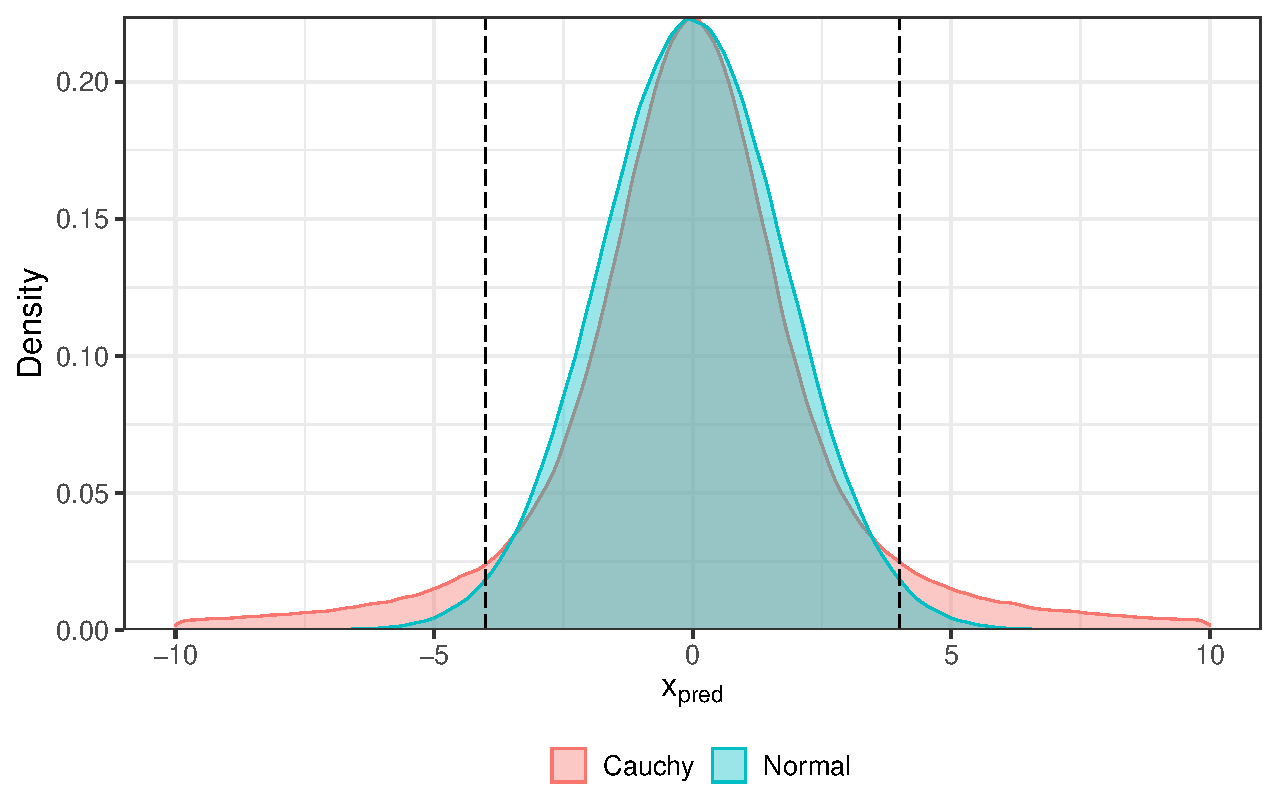
\includegraphics[scale=0.5]{figures/BC_example_326.pdf}
 \caption{Prior predictive distributions of $x$ under Normal and Cauchy priors.}
\end{figure}
\end{frame}
%%%%%%%%%%%%%%%%%%%%%%%%%%%%%%%%%%%
\begin{frame}{Conjugacy}
Conjugacy is a central concept in Bayesian statistics. 
It provides a functional view of the prior-posterior mechanic that emphasises tractability over coherence.
\begin{defn}[Conjugate]
\label{def:conjugate}
A family $\mathcal{F}$ of distributions on $\boldsymbol{\Theta}$ is called \textbf{conjugate} or closed under sampling for a likelihood $f(x \mid \theta)$ if, for every $\pi \in \mathcal{F}$, $p(\theta \mid x) \in \mathcal{F}$.
\end{defn}
\textbf{Arguments for using conjugate priors}
\begin{itemize}
 \item ``Form-preservation'': in a limited-information setting it makes sense that $p(\theta \mid x)$ and $\pi(\theta)$ lie on the same family, since the information in $x$ might not be enough to change the structure of the model, just its parameters;
 \item Simplicity: when you do not know a whole lot, it makes sense to KISS\footnote{Keep it simple, stupid!};
 \item Sequential learning: since $\mathcal{F}$ is closed under sampling, one can update a sequence of posteriors $p_i(\theta \mid x_1, \ldots, x_i)$ as data comes in.
\end{itemize}
\end{frame}
%%%%%%%%%%%%%%%%%%%%%%%%%%%%%%%%%%%
\begin{frame}{Exponential families}
The exponential family of distributions is a cornerstone of statistical practice, underlying many often-used models. 
Here are a few useful definitions.
\begin{defn}[(Natural) Exponential family]
 \label{def:expo_family}
 Let $\mu$ be a $\sigma$-finite measure on $\mathcal{X}$ and let $\boldsymbol{\Theta}$ be a non-empty set serving as the parameter space.
 Let $C : \boldsymbol{\Theta} \to (0, \infty)$ and $h: \boldsymbol{\Theta} \to (0, \infty)$ and let $R : \boldsymbol{\Theta} \times \mathcal{X} \to \mathbb{R}^k$ and $T: \boldsymbol{\Theta} \times \mathcal{X} \to \mathbb{R}^k$.
 The family of distributions with density 
 \begin{equation*}
  f(x \mid \theta) = C(\theta)h(x)\exp\left(R(\theta) \cdot T(x) \right)
 \end{equation*}
 w.r.t. $\mu$ is called an \textbf{exponential family}.
 Moreover, if $R(\theta) = \theta$, the family is said to be \textbf{natural}.
\end{defn}
\begin{defn}[Regular exponential family]
 We say a natural exponential family $f(x\mid\theta)$ is \textbf{regular} if the natural parameter space
 \begin{equation}
  N := \left\{ \theta : \int_{\mathcal{X}} \exp(\theta\cdot x) h(x)\,d\mu(x) < \infty \right\},
 \end{equation}
is an open set of the same dimension as the closure of the convex hull of $\supp(\mu)$.
\end{defn}
\end{frame}
%%%%%%%%%%%%%%%%%%%%%%%%%%%%%%%%%%%
\begin{frame}{Conjugacy and sufficiency}
There is an intimate link between sufficiency (i.e. the existence of sufficient statistics) and conjugacy.
The following is a staple of Bayesian theory.
\begin{theo}[Pitman-Koopman-Darmois]
 If a family of distributions $f(\cdot \mid \theta)$ whose support does not depend on $\theta$ is such that, for a sample size large enough, there exists a sufficient statistic of \underline{fixed dimension}, then $f(\cdot \mid \theta)$ is an exponential family.
\end{theo}
The support condition is not a complete deal breaker, however:
\begin{remark}[Quasi-exponential]
 The $\operatorname{Uniform}(-\theta, \theta)$ and $\operatorname{Pareto}(\theta, \alpha)$ families are called \textit{quasi-exponential} due to the fact that there do exist sufficient statistics of fixed dimension for these families, even though their supports depend on $\theta$.
\end{remark}
\end{frame}
%%%%%%%%%%%%%%%%%%%%%%%%%%%%%%%%%%%
\begin{frame}{Conjugacy in the exponential family}
I hope you are convinced of the utility of the exponential family by now.
It would be nice to have an automated way to deduce a conjugate prior for $f(x\mid \theta)$ when it is in the exponential family.
This is exactly what the next result gives us.
\begin{remark}[Conjugate prior for the exponential family]
 A conjugate family for $f(x\mid \theta)$ is given by
 \begin{equation}
 \label{eq:conjugate_exponential_family}
  \pi(\theta \mid \mu, \lambda) = K(\mu, \lambda) \exp\left(\theta \cdot \mu - \lambda g(\theta)\right),
 \end{equation}
such that the posterior is given by $p(\theta \mid \mu + x, \lambda + 1)$.
\end{remark}
Please do note that (\ref{eq:conjugate_exponential_family}) is only a valid density when $\lambda > 0$ and $\mu/\lambda$ belongs to the interior of the natural space parameter. 
Then, it is a $\sigma$-finite measure.
See \cite{Diaconis1979} for more details.
\end{frame}

%%%%%%%%%%%%%%%%%%%%%%%%%%%%%%%%%%%
\begin{frame}{Conjugacy: common families}
\begin{figure}
 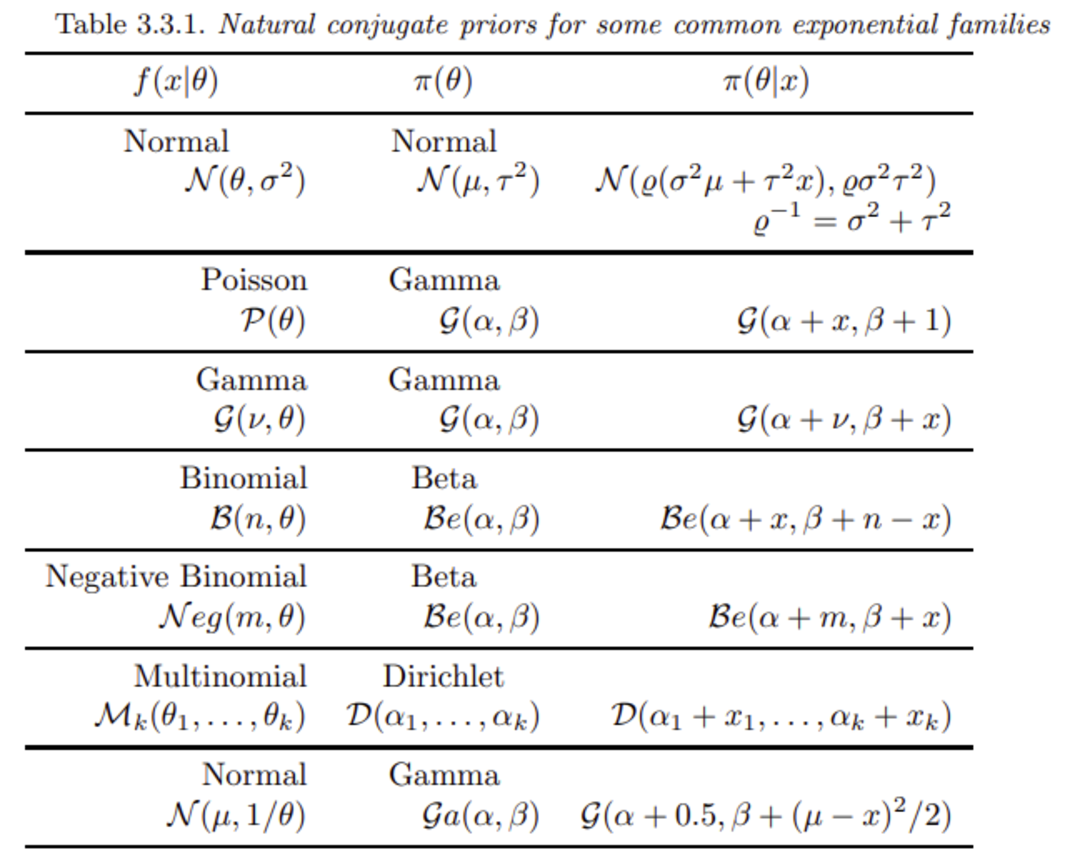
\includegraphics[scale=.5]{figures/conjugate_table.pdf}
 \caption{Taken from~\cite{Robert2007}, page 121.}
\end{figure}
\end{frame}
%%%%%%%%%%%%%%%%%%%%%%%%%%%%%%%%%%%
\begin{frame}{Conjugacy: drawbacks}
Conjugate modelling is certainly useful, but has its fair share of pitfalls.

\textbf{Arguments against using conjugate priors}
\begin{itemize}
 \item Conjugate priors are restrictive \textit{a priori}: in many settings, specially in high dimensions, the set of conjugate priors that retain tractability is so limited so as to not be able to encode all prior information available;
 \item Conjugate priors are not truly subjective: they limit the analyst's input to picking values for the hyperparameters;
  \item Conjugate priors are restrictive \textit{a posteriori}: you are stuck with a given structure forever, no matter how much data you run into.
\end{itemize}
\end{frame}
%%%%%%%%%%%%%%%%%%%%%%%%%%%%%%%%%%%
\begin{frame}{The principle of insufficient reason}
 Also called principle of indifference by Keynes\footnote{John Maynard Keynes (1883--1946) was an English economist.}.
 \begin{quote}
  ...if there is no known reason for predicating of our subject one rather than another of several alternatives, then relatively to such knowledge the assertions of each of these alternatives have an equal probability." \cite[Ch4 pg. 52-53]{Keynes1921}. 
 \end{quote}
 The idea dates back to Laplace and even Bayes himself and usually leads to 
$$ \pi(\theta) \propto 1.$$
 \end{frame}
%%%%%%%%%%%%%%%%%%%%%%%%%%%%%%%%%%%
\begin{frame}{Invariance}
In many applications we might want some sort of~\textit{invariance} in our prior model. 
\begin{defn}[Invariant model]
 \label{def:invariant_model}
 A statistical model is said to be~\textbf{invariant} (or closed) under the action of a group $\mathcal{G}$ if $\forall g \in \mathcal{G} \: \exists \theta^\star \in \boldsymbol{\Theta}$ such that $y = g(x)$ is distributed with density $f(y\mid \theta^\star)$, denoting $\theta^\star = \bar{g}(\theta)$.
\end{defn}
Consider two types of invariance
\begin{itemize}
 \item \textit{Translation} invariance:
 A model $f(x-\theta)$ such that $x-x_0$ has a distribution in the same family for every $x_0$ leads to
 $$\pi(\theta) = \pi(\theta-\theta_0),\: \forall\: \theta_0 \in \boldsymbol{\Theta}.$$
 \item \textit{Scale} invariance:
 Similarly, a model of the form $\sigma^{-1} f(x/\sigma)$, $\sigma >0$ is \textit{scale-invariant} and  leads to
 $$ \pi(A/c) = \pi(A),$$
 for any measurable A.
\end{itemize}
\end{frame}
%%%%%%%%%%%%%%%%%%%%%%%%%%%%%%%%%%
\begin{frame}{Jeffreys's prior}
One can try to build a prior that captures only the essential structural information about the problem by deriving an invariant distribution from the Fisher information:
$$ I(\theta) = E\left[\left(\frac{\partial \log f(X \mid \theta)}{\partial \theta}\right)^2\right].$$
Under regularity conditions, we can usually also write
$$ I(\theta) = - E\left[\frac{\partial^2 \log f(X \mid \theta)}{\partial \theta^2}\right].$$
Jeffreys showed that 
$$\pi_J(\theta) \propto \sqrt{I(\theta)},$$
is invariant.
There are straightforward generalisations when $\theta$ is multidimensional.
\end{frame}
%%%%%%%%%%%%%%%%%%%%%%%%%%%%%%%%%%
\begin{frame}{Jeffreys's priors: examples}
A good exercise is to show that
\begin{itemize}
 \item If $x \sim \operatorname{Normal}(0, \theta)$, $\pi_J(\theta) \propto 1/\theta^2$;
 \item If $x \sim \operatorname{Normal}_d(\theta, \boldsymbol{I}_d)$, $\pi_J(\theta) \propto 1$;
 \item If $x \sim \operatorname{Binomial}(n, \theta)$, $\pi_J(\theta) \equiv \operatorname{Beta}(1/2, 1/2)$;
 \item If $f(x\mid \theta) = h(x) \exp\left(\theta \cdot x - \psi(\theta)\right)$, then
 $$ \pi_J(\theta)  \propto \sqrt{\prod_{i=1}^k\psi^{\prime\prime}(\theta)}.$$
\end{itemize}
\end{frame}
%%%%%%%%%%%%%%%%%%%%%%%%%%%%%%%%%%
\begin{frame}{Beware!}
One important caveat of Jeffreys's priors is that they violate the Likelihood Principle.
To see why, consider the following exercise.
\begin{exercise}[Poisson process]
Suppose one is interested in estimating the rate, $\theta$, of a Poisson process:
$$ Y(t) \sim \operatorname{Poisson}(t\theta).$$
There are two possible experimental designs: 
\begin{itemize}
 \item[a)] Fix a number $n$ of events to be observed and record the time $X$ to observe them, or;
 \item[b)] Wait a fixed amount of time, $t$, and count the number $Y$ of occurences of the event of interest.
 Show that
\end{itemize}
 \begin{align*}
\label{eq:poisson_process_informationMatrix}
\text{a)}&\:  I_X(\theta) = \frac{n}{\theta^2},\\
\text{b)}&\: I_Y(\theta) = \frac{t}{\theta}.
\end{align*}
Which conclusions can we draw from this example?
\end{exercise}
See also example 3.5.7 in~\cite{Robert2007}.
\end{frame}
%%%%%%%%%%%%%%%%%%%%%%%%%%%%%%%%%%
\begin{frame}{Reference priors}
Jeffreys's approach can sometimes lead to marginalisation paradoxes and calibration issues (see exercise 4.47 in \cite{Robert2007}).
\cite{Bernardo1979} proposes a modification that avoids these difficulties by explicit separating parameters in~\textit{nuisance} and~\textit{interest}.
It works like this: take $f(x\mid \theta)$, with $\theta = (\theta_1, \theta_2)$ and let $\theta_1$ be the parameter of interest.
We must first compute\footnote{Notice that this need not be well-defined. One common way of dealing with difficulties is to integrate on a sequence of measurable compact sets and take the limit.}
$$ \tilde{f}(x\mid \theta_1) = \int_{\boldsymbol{\Theta_2}} f(x \mid \theta_1, t_2)\pi(t_2\mid \theta_1)\, dt_2, $$
and then compute the Jeffreys's prior associated with this marginalised likelihood.
Notice that this entails first deriving $\pi(\theta_2\mid \theta_1)$.
\end{frame}
%%%%%%%%%%%%%%%%%%%%%%%%%%%%%%%%%%
\begin{frame}{Reference priors: example}
Suppose we have $x_{ij} \sim \operatorname{Normal}(\mu_i, \sigma^2)$, $i = 1, \ldots, n$, $j=1,2$ and consider making inferences about $\boldsymbol{\theta} = (\sigma^2, \boldsymbol{\mu})$.
Here $\theta_1 = \sigma$ is a nuisance parameter and we're interested in the location $\boldsymbol{\theta}_2 = \boldsymbol{\mu}$.
The Jeffreys's prior is 
$$\pi_J(\boldsymbol{\theta}) \propto 1/\sigma^{n+1},$$
leading to a Bayes estimator under quadratic loss:
$$ \hat{\sigma}_J := E[\sigma^2 \mid \boldsymbol{x}] = \frac{\sum_{i=1}^n (x_{i1}-x_{i2})^2}{4n-4},$$
which in not consistent.
The reference approach give $\pi(\theta_1 \mid \boldsymbol{\theta_2})$ as a flat prior - because $\boldsymbol{\theta_2}$ is a location parameter.
Marginalising the likelihood against this flat density over $(0,\infty)$ gives $\pi_R(\sigma^2) \propto 1/\sigma^2$, leading to
$$ \hat{\sigma}_R =\frac{\sum_{i=1}^n (x_{i1}-x_{i2})^2}{2n-4},$$
which is consistent.
Phew!
\end{frame}
%%%%%%%%%%%%%%%%%%%%%%%%%%%%%%%%%%
\begin{frame}{Frequentist considerations}
If you are a bit greedy and want to please Greeks and Troyans, you might also try to construct your prior so that it attains good frequency properties. 
One such way is to construct~\textbf{matching priors}:
\begin{defn}[Matching prior]
 We say $\pi(\theta)$ is a \textbf{matching prior} for a confidence level $\alpha$ if it is constructed in such a way that  
 \begin{equation*}
  \pr(g(\theta) \in C_x \mid x) = \frac{1}{m(x)}\int_{C_x} f(x\mid t) \pi(t) \, dt = 1-\alpha,
 \end{equation*}
holds for a given confidence set $C_x(\alpha)$ for $g(\theta)$.
\end{defn}
In other words, if the posterior matches the confidence set.
It can be shown that, in unidimensional families, the Jeffreys's prior gives
$$ \pr(\theta \leq k_\alpha(x)) = 1-\alpha + O(n^{-1}),$$
where $C_x = (-\infty, k_\alpha(x))$ is a one-sided confidence interval.
\end{frame}
%%%%%%%%%%%%%%%%%%%%%%%%%%%%%%%%%%
\begin{frame}{Prior classes}
\cite{Robert2007} gives a classification of priors in classes:
\begin{itemize}
 \item[i)] Conjugate classes:
  $$ \Gamma_C = \{\pi \in \mathcal{F} : p \in \mathcal{F} \}, $$
 \item[ii)] Determined moment(s) classes:
 $$ \Gamma_M = \{\pi : a_i \leq E_\pi[\theta] \leq b_i, i = 1, \ldots, k\}, $$
 \item[iii)] Neighbourhood (or $\epsilon$-contamination) classes:
  $$ \Gamma_{\epsilon, \mathcal{Q}} = \{\pi = (1-\epsilon)\pi_0 + q, q \in \mathcal{Q}\}, $$
 \item[iv)] Underspecified classes:
   $$ \Gamma_{U} = \{\pi : \int_{I_i} \pi(t)\,dt \leq \mu_i, i = 1, \ldots, k\}, $$
 \item[v)] Ratio of density classes:
    $$ \Gamma_{R} = \{\pi : L(\theta) \leq \pi(\theta) \leq U(\theta)\}. $$
\end{itemize}
\end{frame}
%%%%%%%%%%%%%%%%%%%%%%%%%%%%%%%%%%
\begin{frame}{Prior sensitivity analysis}
 General recommendations about building priors:
 \begin{itemize}
  \item Check the \textbf{observable consequences} of your priors :what kinds of data does this produce?
  \item Check the inferential consequences of your priors: how do my estimators change under different priors?
  \item Make sure you know what your restrictions do to the tail of your prior;  
  \item It is usually a good idea to understand what the prior \textbf{does} to the model, as opposed to only which values $\theta$ can plausibly take;
  \item Sometimes it may be useful to think of priors as \textit{penalisations} that \textbf{regularise} inference.
 \end{itemize}
\end{frame}

%%%%%%%%%%%%%%%%%%%%%%%%%%%%%%%%%%
\begin{frame}{Recommended reading}
\begin{itemize}
 \item[\faBook] \cite{Robert2007} Ch. 3;
 \item[\faForward] Next lecture: \cite{Robert2007} Ch. 3.6, \cite{Seaman2012}, \cite{Gelman2017} and \cite{Simpson2017}.
 \end{itemize} 
\end{frame}

\section*{Bayesian point estimation}
\begin{frame}{The maximum~\textit{a posteriori} (MAP) estimator}
\begin{defn}[Maximum~\textit{a posteriori}]
The posterior mode or maximum~\textit{a posteriori} (MAP) estimator of a parameter $\theta$ is given by
\begin{equation}
 \label{eq:MAP}
 \delta_{\pi}^{\text{MAP}}(x) := \argmax_{\theta \in \boldsymbol{\Theta}} p(\theta \mid x).
\end{equation}
\end{defn}
\begin{example}[MAP for the binomial case]
 Suppose $x \sim \operatorname{Binomial}(n, p)$.
 Now consider the following three priors for $p$: 
 \begin{itemize}
  \item $\pi_0(p) = \frac{\sqrt{p(1-p)}}{B(1/2, 1/2)} $ [Jeffreys];
  \item $\pi_1(p) = 1$ [Beta(1,1)/Uniform];
  \item $\pi_2(p) = \left(p(1-p)\right)^{-1}$ [\cite{Haldane1932}].  
 \end{itemize}
These lead to 
\begin{itemize}
 \item $\delta_0^{\text{MAP}}(x) = \max \{(x-1/2)/(n-1), 0 \}$;
 \item $\delta_1^{\text{MAP}}(x) = x/n$;
 \item $\delta_2^{\text{MAP}}(x) = \max \{ (x-1)/(n-2), 0 \}$.
\end{itemize}
\end{example}
\end{frame}
%%%%%%%%%%%%%%%%%%%%%%%%%%%%%%%%%%%
\begin{frame}{A word of caution}
 We end this discussion with the following warning:
\begin{idea}[Marginalise, not maximise]
\label{idea:always_marginalise}~
 Bayesian approaches to estimation and prediction \underline{usually} focus on \textit{marginalisation} rather than \textit{optmisation}.
 This is because, following the Likelihood Principle, all of the information available about the unknowns is contained in the posterior distribution, and thus all inferences must be made using this probability measure, usually by finding suitable expectations of functionals of interest.
\end{idea}
In particular, for higher dimensions, \textbf{concentration of measure}\footnote{See these excellent notes by Terence Tao:\url{https://terrytao.wordpress.com/2010/01/03/254a-notes-1-concentration-of-measure/} .} ensures that the posterior mode has less and less relevance as a summary, at least so far as the barycentre of the distribution is concerned.
\end{frame}
%%%%%%%%%%%%%%%%%%%%%%%%%%%%%%%%%%%
\begin{frame}{Precision of Bayes estimators}
 A central quantity in the evaluation of Bayesian estimators is
 \begin{equation}
  \label{eq:bayes_risk}
  E_p\left[\left(\delta_\pi - h(\theta)\right)^2\right] = E_{\pi}\left[\left(\delta_\pi - h(\theta)\right)^2 \mid x \right]
 \end{equation}
for measurable $h$.
\begin{example}[Bayes versus frequentist risk]
 Take $x \sim \operatorname{Binomial}(n, \theta)$ with $n$ known and place a Jeffreys's prior on $\theta$.
 Consider the MLE: $\delta_1(x) = x/n$.
 It can be shown that:
 $$ E_\pi\left[\left(\delta_1 - \theta \right)^2 \mid x \right] = \left(\frac{x - n/2}{n(n+1)}\right)^2 +  \frac{(x + 1/2)(n - x + 1/2)}{(n + 1)^2(n+2)}.$$
 Moreover,
 $$\argmax_{\theta \in (0, 1)}  E_\pi\left[\left(\delta_1 - \theta\right)^2 \mid x \right] = [4(n+2)]^{-1},$$
 and
 $$ \argmax_{\theta \in (0, 1)} E_\theta \left[\left(\delta_1 - \theta\right)^2\right] = [4n]^{-1}.$$ 
\end{example}
\end{frame}
%%%%%%%%%%%%%%%%%%%%%%%%%%%%%%%%%%%
\begin{frame}{A brief aside about prediction}
 Prediction is an important inferential task and is somewhat related to the previous discussion on precision.
 Consider predicting a quantity $z$ \textbf{conditional} on data $x$.
 For that  we need $g(z \mid x, \theta)$, $f(x\mid \theta)$ and $\pi(\theta)$.
 Then,
 \begin{equation}
  \label{eq:general_predictive}
  g_\pi(z\mid x) = \int_{\boldsymbol{\Theta}} g(z\mid x, t) p(t \mid x)\,dt
 \end{equation}
encodes all of the information brought by the posterior about $z$.
A special case  is i.i.d prediction:
\begin{equation}
 \label{eq:posterior_predictive_data}
 g(\tilde{x} \mid x) = \int_{\boldsymbol{\Theta}} f(\tilde{x} \mid t) p(t \mid x)\,dt
\end{equation}
is the posterior predictive of the new data $\tilde{x}$.
\begin{idea}[Calibrated priors for prediction]
\label{idea:prediction_calibrated_priors}
The prior, $\pi$, can be constructed so as to minimise error in a prediction task. 
\end{idea}
\end{frame}
%%%%%%%%%%%%%%%%%%%%%%%%%%%%%%%%%%%
\begin{frame}{A neat trick}
Computing expectations all the time means we have to become familiar with a few tricks to facilitate obtaining approximate answers.
\begin{example}[Mixture representation of the Student-t]
Take $x \sim \operatorname{Normal}_p(\theta, \boldsymbol{I}_p)$ and put $\theta \sim \operatorname{Student-t}_p(\alpha, 0, \tau^2\boldsymbol{I}_p)$.
Then $p(\theta \mid x)$ does not have a closed-form normalising constant and computing the Bayes estimator under quadratic loss is a chore.
However, we can use the representation
\begin{align*}
 \theta \mid z &\sim \operatorname{Normal}_p(0, \tau^2z\boldsymbol{I}_p),\\
 z & \sim \operatorname{InverseGamma}(\alpha/2, \alpha/2),
\end{align*}
to get 
$$ \theta \mid x, z \sim  \operatorname{Normal}_p\left(\frac{x}{ 1+ \tau^2z}, \frac{\tau^2z}{ 1+ \tau^2z}\boldsymbol{I}_p\right) $$ 
Thus, the Bayes estimator $\delta_\pi(x) = \int_0^\infty E_\pi[\theta \mid x, z]p(z \mid x)\,dz$ can be computed with a single integral for any dimension $p$. 
\end{example} 
\end{frame}
%%%%%%%%%%%%%%%%%%%%%%%%%%%%%%%%%%%
\begin{frame}{Conjugacy is handy!\footnote{Taken from~\cite{Robert2007}.}}
\begin{center}
 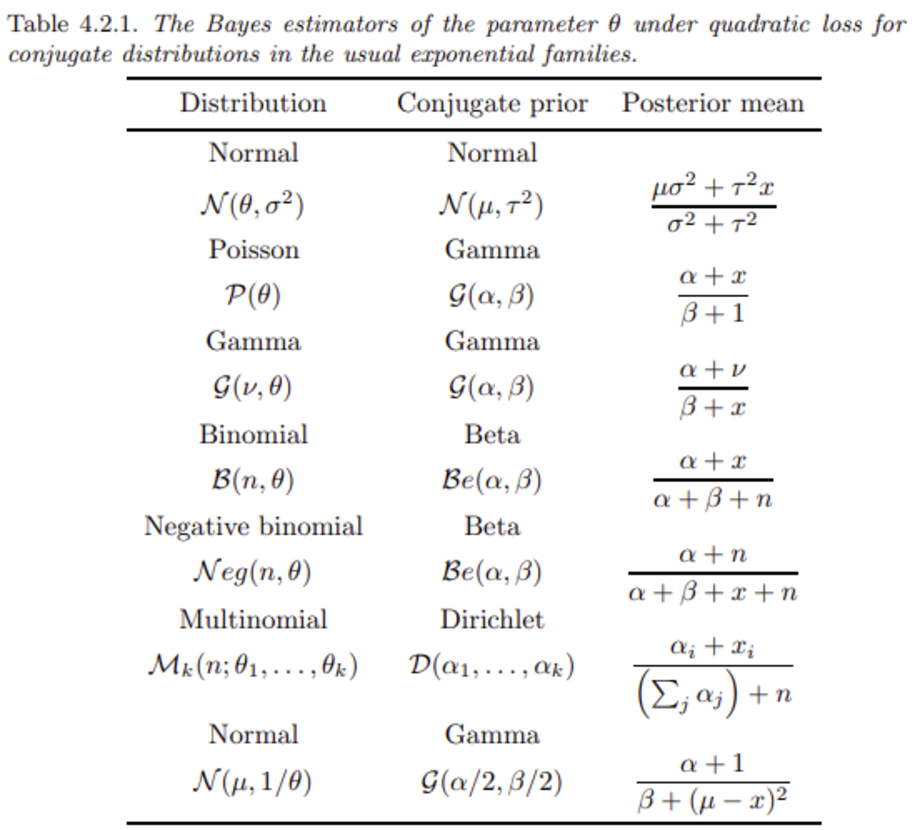
\includegraphics[scale=0.5]{figures/conjugate_table_expectations.pdf}
\end{center}
\end{frame}
%%%%%%%%%%%%%%%%%%%%%%%%%%%%%%%%%%%
\begin{frame}{A worked example}
We will stretch our Bayesian muscles with the next problem. 
\begin{exercise}[Inference for the rate of a Gamma]
\label{exercise:rate_gamma_different_losses}
 Let $x \sim \operatorname{Gamma}(\nu, \theta)$ with $\nu >0$ known.
 A natural choice of prior is $\theta \sim \operatorname{Gamma}(\alpha, \beta)$.
 Find the Bayes estimator under 
 $$ L_1(\delta, \theta) = \left(\delta - \frac{1}{\theta}\right)^2, $$
 and the scale-invariant loss
 $$ L_2(\delta, \theta) = \theta^2 \left(\delta - \frac{1}{\theta}\right)^2$$
 \textit{Hint:} If $X \sim \operatorname{Gamma}(\alpha, \beta)$, $Y = 1/X \sim \operatorname{InverseGamma}(\alpha, \beta)$ and $E[Y^k] = \frac{\beta}{(\alpha-1)\cdots(\alpha-k)}$
\end{exercise}
\end{frame}
%%%%%%%%%%%%%%%%%%%%%%%%%%%%%%%%%%%
\begin{frame}{A quick note on quadratic loss}
 Exercise~\ref{exercise:rate_gamma_different_losses} is a special case of the general situation where 
 $$ L(\delta, \theta) = w(\theta) ||\delta-\theta||_{\boldsymbol{G}}^2, $$
 for $\boldsymbol{G}$ a $p \times p$ non-negative symmetric matrix.
 In this case, we get
 $$ \delta_\pi = \frac{E_p[w(\theta)\theta]}{E_p[w(\theta)]}. $$
 Please \textbf{note} that there is no universal justification for quadratic loss other than (sometimes leading to increased) mathematical tractability
\end{frame}
%%%%%%%%%%%%%%%%%%%%%%%%%%%%%%%%%%%
\begin{frame}{Loss estimation}
 Since the loss function, $L(\delta(x), \theta)$ is usually measurable w.r.t the posterior, it can be estimated much the same way as other functionals.
 In particular, if you are feeling particularly eclectic, you can always constructed $\pi$ such that
 $$ E\left[E_p[L(\delta_\pi(x), \theta]\right] \geq R(\delta_\pi(x), \theta),  \theta \in \boldsymbol{\Theta}, $$
 i.e. that the estimated loss never underestimates the error resulting from the use of $\delta_\pi$, at least in the long run.
 This is called \textbf{frequentist validity}.
 \end{frame}
%%%%%%%%%%%%%%%%%%%%%%%%%%%%%%%%%%%
\begin{frame}{A nice little problem by Neyman}
The following problem is described by Jeffreys as originating with Jerzy Neyman\footnote{Jerzy Neyman (1894-1981) was a Polish-American statistician, known for with work with Egon Pearson (1895-1980) on the foundations of the null hypothesis significance testing (NHST) framework.}.
\begin{exercise}[The tramcar problem]
 \label{exercise:tramcar}
 A person travelling in a a foreign country has to change trains at a junction, and goes into the town, the existence of which they have only just heard.
 They have no idea of its size.
 The first thing they see is a tramcar numbered $100$.
 Assuming tramcars are numbered consecutively from $1$ onwards, what could one \textit{infer} about the number $N$ of tramcars in this town?
\end{exercise}

\end{frame}

%%%%%%%%%%%%%%%%%%%%%%%%%%%%%%%%%%%
\begin{frame}{Recommended reading}
\begin{itemize}
  \item[\faBook] \cite{Robert2007}, Ch4.
%  \item 
 \item[\faForward] Next lecture: \cite{Robert2007} Ch. 5.
 \end{itemize} 
\end{frame}

\section*{Bayesian teting and ``interval'' estimation}
%%%%%%%%%%%%%%%%%%%%%%%%%%%%%%%%%%%
\begin{frame}{The duality between estimation and testing}
Similarly to the frequentist case, in Bayesian inference there is an intimate relationship between testing hypotheses an estimating measurable functions of the parameters.
\begin{defn}[Test]
 Consider a statistical model $f(x \mid \theta)$  with $\theta \in \boldsymbol{\Theta}$. 
 Given $\boldsymbol{\Theta}_0 \subset \boldsymbol{\Theta}$, a \textit{test} consists in answering the question of whether
 $$ H_0 : \theta \in \boldsymbol{\Theta}_0 $$
 is true.
 We call $H_0$ the \textit{null hypothesis} and $\boldsymbol{\Theta}_0$ can often be a point, i.e. $\boldsymbol{\Theta}_0 = \{\theta_0 \}$.
\end{defn}
Notice that $\mathbb{I}_{\boldsymbol{\Theta}_0}(\theta)$ is measurable and thus we can define, for instance
\begin{equation*}
L_1(\theta, \varphi) = \begin{cases}
1, \varphi = \mathbb{I}_{\boldsymbol{\Theta}_0}(\theta),\\
0, \: \text{otherwise},
\end{cases}
\end{equation*}
which in turn leads to 
\begin{equation*}
\varphi_1 = \begin{cases}
1, \pr(\theta \in \boldsymbol{\Theta}_0 \mid x) > \pr(\theta \in \boldsymbol{\Theta}_0^c \mid x),\\
0, \: \text{otherwise}.
\end{cases}
\end{equation*}
\end{frame}
%%%%%%%%%%%%%%%%%%%%%%%%%%%%%%%%%%%
\begin{frame}{A refinement}
 The loss function just seen can be refined to
 \begin{equation*}
L_2(\theta, \varphi) = \begin{cases}
0, \varphi = \mathbb{I}_{\boldsymbol{\Theta}_0}(\theta),\\
a_0, \theta \in \boldsymbol{\Theta}_0, \varphi = 0\\
a_1, \theta \in \boldsymbol{\Theta}_0^c, \varphi = 1.
\end{cases}
\end{equation*}
Under this loss, we have
\begin{equation*}
\varphi_2 = \begin{cases}
1, \pr(\theta \in \boldsymbol{\Theta}_0 \mid x) >  a_1/(a_0 + a_1),\\
0, \: \text{otherwise}.
\end{cases}
\end{equation*}
\end{frame}
%%%%%%%%%%%%%%%%%%%%%%%%%%%%%%%%%%%
\begin{frame}{Example}
\begin{example}[\textit{One} Normal test]
  Take, for example, $x \sim \operatorname{Normal}(\theta, \sigma^2)$, with $\theta \sim \operatorname{Normal}(\mu_0, \tau^2)$.
This implies $\theta \mid x \sim \operatorname{Normal}(\mu(x), \omega^2)$, where
\begin{align*}
 \mu(x) &= \frac{\sigma^2\mu_0 + \tau^2x}{\sigma^2 + \tau^2};
 \omega^2 = \frac{\sigma^2\tau^2}{\sigma^2 + \tau^2}.
\end{align*}
To test $H_0: \theta < 0$, we can compute
\begin{align*}
 \pr(\theta < 0 \mid x) &= \pr \left(\frac{\theta-\mu(x)}{\omega} < \frac{\mu(x)}{\omega}\right), \\
 &= \Phi\left(\frac{-\mu(x)}{\omega}\right).
\end{align*}
This means that if $z_{a_0, a_1}$ is such that $\Phi(z_{a_0, a_1}) = a_1/(a_0 + a_1)$, we can accept $H_0$ if 
$$\mu(x) < -z_{a_0, a_1}\omega. $$
\end{example}
\end{frame}
%%%%%%%%%%%%%%%%%%%%%%%%%%%%%%%%%%%
\begin{frame}{Bayes factors}
A central tool in Bayesian testing is the \textbf{Bayes factor} -- see \cite{Kass1995} for a review and guide for interpretation.
\begin{defn}[Bayes factor]
 \label{def:Bayes_factor}
 The Bayes factor is the ratio of posterior odds and the prior odds over the null and the alternative:
 \begin{align*}
  B^\pi_{01}(x) &= \frac{\pr(\theta \in\boldsymbol{\Theta}_0 \mid x)}{\pr(\theta \in\boldsymbol{\Theta}_1 \mid x)}\bigg/\frac{\pr(\theta \in\boldsymbol{\Theta}_0)}{\pr(\theta \in\boldsymbol{\Theta}_1)},\\
  &= \frac{\pr(\theta \in\boldsymbol{\Theta}_0 \mid x)\cdot\pr(\theta \in\boldsymbol{\Theta}_1)}{\pr(\theta \in\boldsymbol{\Theta}_1 \mid x)\cdot\pr(\theta \in\boldsymbol{\Theta}_0)}.
 \end{align*}
\begin{remark}
 When $\boldsymbol{\Theta}_0 = \{\theta_0\}$ and  $\boldsymbol{\Theta}_1 = \{\theta_1\}$ the Bayes factor simplifies to
 \begin{equation*}
  r_{01}(x) = \frac{f(x\mid\theta_0)}{f(x\mid\theta_1)},
 \end{equation*}
 also known as the \textbf{likelihood ratio}.
\end{remark}
\end{defn}
\end{frame}
%%%%%%%%%%%%%%%%%%%%%%%%%%%%%%%%%%%
\begin{frame}{A few more considerations on the Bayes factor}
The Bayes factor can also be written as 
\begin{align*}
  B^\pi_{01}(x) &=  \frac{\int_{\boldsymbol{\Theta}_0} f(x\mid t)\pi_0(t)\,dt }{\int_{\boldsymbol{\Theta}_1} f(x\mid t)\pi_1(t)\,dt} = \frac{m_0(x)}{m_1(x)},
\end{align*}
where $\pi_0$ and $\pi_1$ are the prior distributions under each hypothesis.
Also, if $\hat{\theta}_0$ and $\hat{\theta}_1$ are the MLE under each hypothesis, by making $\pi_0$ and $\pi_1$ Dirac masses at $\hat{\theta}_0$ and $\hat{\theta}_1$, respectively, we recover
\begin{equation}
\label{eq:bayes_lrt}
 R(x) = \frac{\sup_{\theta \in \boldsymbol{\Theta}_0}f(x \mid \theta)}{\sup_{\theta \in \boldsymbol{\Theta}_1}f(x \mid \theta)}
\end{equation}
\begin{exercise}[Bayesian justifcation of LRT]
 Does (\ref{eq:bayes_lrt}) offer a Bayesian justifcation for likelihood ratios?
\end{exercise}
\end{frame}
%%%%%%%%%%%%%%%%%%%%%%%%%%%%%%%%%%%
\begin{frame}{Testing point-null hypotheses}
Hypotheses of the form $H_i : \theta \in \{ \theta_i \}$, called point-null hypotheses, are hard to deal with from a probabilistic point of view.
\begin{remark}[Point-null hypotheses under continuous priors]
 Point-null cannot be tested under continuous prior distributions.
 More generally, if either $H_0$ or $H_1$ are \textbf{impossible} \textit{a priori}, then no amount of data can change that belief.
\end{remark}
\begin{idea}[Cromwell's law\footnote{This idea is attributed to British statistician Dennis Lindley (1923-2013), one of the founders of modern Bayesian theory.}]
 In general, one not assign probability zero to events that are not logically or physically demonstrably impossible.
 Or, more eloquently, as  Oliver Cromwell writes to the General Assembly of the Church of Scotland on 3 August 1650:
 \begin{quotation}
  I beseech you, in the bowels of Christ, think it possible that you may be mistaken.
 \end{quotation}
\end{idea} 
\end{frame}
%%%%%%%%%%%%%%%%%%%%%%%%%%%%%%%%%%%
\begin{frame}{Point-null hypotheses: modification of the prior}
Testing point-null hypotheses involves a \textbf{modification of the prior}
 If $H_0: \theta \in \{\theta_0\}$  we can write $\rho_0 = \pr(\theta = \theta_0)$ and then
 \begin{equation*}
  \tilde{\pi}(\theta) = \rho_0 \mathbb{I}_{\boldsymbol{\Theta}_0}(\theta) + (1-\rho_0)\pi_1(\theta),
 \end{equation*}
is our new prior, where $\pi_1$ is the distribution with density $g_1(\theta) \propto \pi(\theta)\mathbb{I}_{\boldsymbol{\Theta}_1}(\theta)$ with respect to the dominating measure on $\boldsymbol{\Theta}_1$. 
This gives a posterior probability
\begin{equation*}
 \tilde{\pi}(\boldsymbol{\Theta}_0 \mid x) = \frac{f(x \mid \theta_0)\rho_0}{f(x \mid \theta_0)\rho_0 + (1-\rho_0)m_1(x)}.
\end{equation*}
where $m_1(x) = \int_{\boldsymbol{\Theta}_1} f(x \mid t)g_1(t)\,dt$.
It can be shown that
\begin{equation*}
 \tilde{\pi}(\boldsymbol{\Theta}_0 \mid x) = \left[1 + \frac{1-\rho_0}{\rho_0}\frac{1}{B^\pi_{01}(x)}\right]^{-1}, 
\end{equation*}
which makes clear the relationship between posterior probabilities and Bayes factors.
\end{frame}
%%%%%%%%%%%%%%%%%%%%%%%%%%%%%%%%%%%
\begin{frame}{Example}
Consider $x \sim \operatorname{Binomial}(n, p)$ and consider testing $H_0: p = 1/2$ against $H_1: p \neq 1/2$. 
Taking $g_1(p) = 1$, we have
\begin{equation*}
  \tilde{\pi}(\boldsymbol{\Theta}_0 \mid x) = \left[1 + \frac{1-\rho_0}{\rho_0}2^n B(x+1, n-x+1)\right]^{-1}.
\end{equation*}
 \begin{center}
 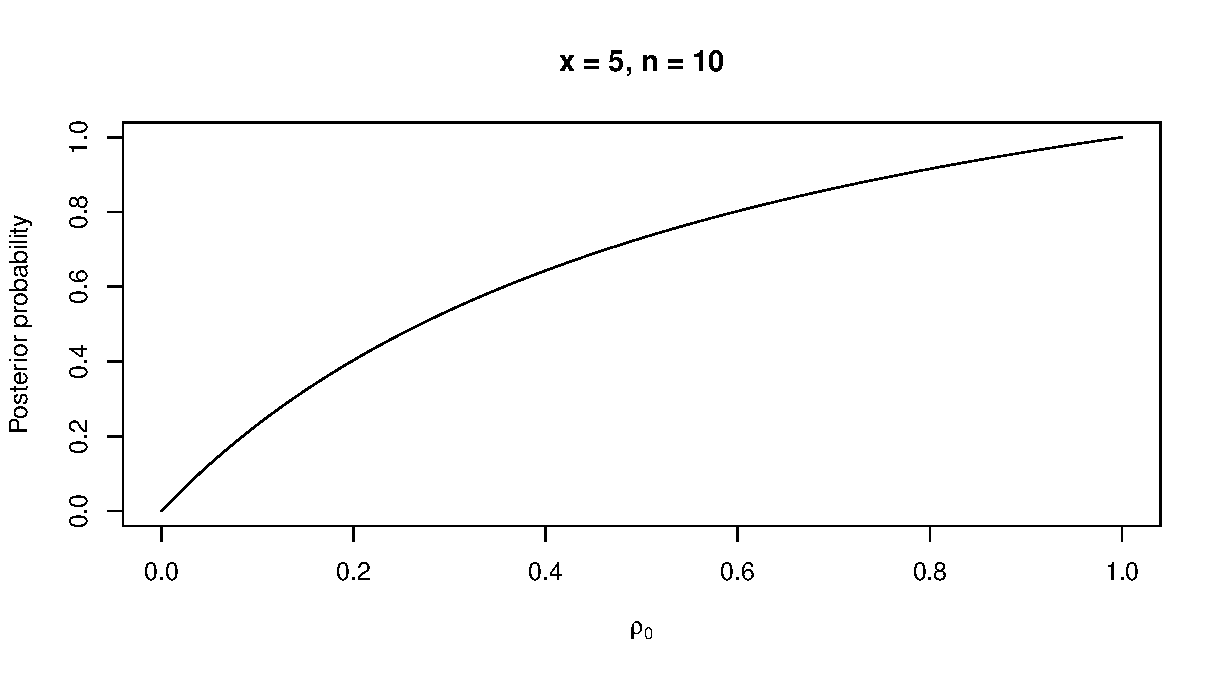
\includegraphics[scale=0.45]{figures/posterior_prob_half.pdf}
\end{center}
\end{frame}
%%%%%%%%%%%%%%%%%%%%%%%%%%%%%%%%%%%
\begin{frame}{Testing with improper priors}
 \begin{idea}[Bayesian hypothesis testing with improper priors]
  No. Just... No.
 \end{idea}
See~\cite{Degroot1973} for the many reasons why this is just a bad idea.
If you insist, please see Section 5.2.5 in \cite{Robert2007} and references therein.
\end{frame}
%%%%%%%%%%%%%%%%%%%%%%%%%%%%%%%%%%%
\begin{frame}{An interesting little paradox}
\begin{idea}[The Jeffreys-Lindley paradox]
Consider $x \sim \operatorname{Normal}(\theta, \sigma^2)$ with $\sigma^2$ known and suppose we are interested in testing $H_0: \theta = \theta_0$ against $H_1: \theta \neq \theta_0$.
We can summarise the data using the sample mean $\bar{x}$ and then compute $t_n = \sqrt{n}(\bar{x}-\theta_0)/\sigma$. 
Employing a conjugate prior $\theta \sim \operatorname{Normal}(\mu_0, \sigma^2)$,
the Bayes factor is
\begin{equation*}
B_{01}(\boldsymbol{x}) = \sqrt{1 + n}\exp\left(-\frac{nt_n^2}{2(1+n)}\right),
\end{equation*}
which goes to infinity with $n$, while the p-value:
\begin{equation*}
 p(t_n) = 1-2\Phi(|t_n|),
\end{equation*}
is constant in $n$.
In practice this means that, for instance $t_n = 1.96$ and $n = 16, 818$, we have 95\% frequentist confidence that $\theta \neq \theta_0$ whilst \textbf{at the same time} having 95\% belief that $\theta = \theta_0$.
\end{idea} 
\end{frame}
%%%%%%%%%%%%%%%%%%%%%%%%%%%%%%%%%%%
\begin{frame}{Another look at principled Bayesian testing}
 Before we were doing
 \begin{equation*}
  L_3(\theta, \varphi) = |\varphi - \mathbb{I}_{\boldsymbol{\Theta}_0}(\theta)|.
 \end{equation*}
But considering a strictly convex loss such as the quadratic loss 
 \begin{equation*}
  L_4(\theta, \varphi) = \left(\varphi - \mathbb{I}_{\boldsymbol{\Theta}_0}(\theta)\right)^2,
 \end{equation*}
 leads to better (more adaptable) estimators in general.
 For instance, the Bayes estimator under $L_4$ is
 \begin{equation*}
  \varphi_\pi(x) = \pr(\theta \in  \boldsymbol{\Theta}_0 \mid x).
 \end{equation*}
 \end{frame}
%%%%%%%%%%%%%%%%%%%%%%%%%%%%%%%%%%%
\begin{frame}{Credibility regions}
After all of this work, we are finally ready to define credibility regions, the main object in Bayesian interval estimation.
\begin{defn}[Credibility region]
For a prior $\pi$, a set $C_x$ is called an $\alpha$-credible set if 
\begin{equation*}
 \pr(\theta \in C_x \mid x) \geq 1-\alpha.
\end{equation*}
We call $C_x$ a highest posterior density (HPD) $\alpha$-credible region if
\begin{equation*}
 \left\{\theta : p(\theta \mid x) > k_\alpha \right\} \subset C_x \subset \left\{\theta : p(\theta \mid x) \geq k_\alpha \right\},
\end{equation*}
subject to the restriction that
\begin{equation*}
 \pr(\theta \in C_x^\alpha) \geq 1-\alpha.
\end{equation*}
\end{defn}
\end{frame}
%%%%%%%%%%%%%%%%%%%%%%%%%%%%%%%%%%%
\begin{frame}{A couple remarks}
Credibility regions have a few desirable properties that make them quite attractive as ``interval'' estimates.
\begin{remark}[No randomisation]
 One nice feature of credibility regions for discrete distributions is that, contrary to the frequentist approach, no randomisation is needed to attain a certain level $\alpha$.
\end{remark}
Also,
\begin{remark}[Improper priors and credibility regions]
 In principle, the use of improper priors poses no problem for the derivation of credibility regions.
\end{remark} 
\end{frame}
%%%%%%%%%%%%%%%%%%%%%%%%%%%%%%%%%%%
\begin{frame}{Credibility regions: Example I}
Sometimes we will be able to provide Bayesian justifcation for frequentist confidence regions/intervals.
\begin{example}[Credibility intervals for the variance in the Normal]
\label{ex:cred_var_normal_Jeffreys}
Consider $\boldsymbol{x} = \{ x_1, \ldots, x_n \}$, $x_i \sim \operatorname{Normal}(\theta, \sigma^2)$, with both parameters unknown.
Consider
$$ \pi(\theta, \sigma^2) \propto \frac{1}{\sigma^2}. $$
Make $s^2 = \sum_{i=1}^n (x-\bar{x})^2$.
It can be shown that $p(\sigma^2 \mid  s^2) \equiv \operatorname{Gamma}(\sigma^2; (n-1)/2, s^2/2)$.
In particular, this implies
\begin{equation*}
 \frac{s^2}{\sigma^2} \mid \bar{x} \sim \operatorname{Chi-square}(n-1),
\end{equation*}
which the attentive student will notice leads to the same solution as the classical confidence approach.
\end{example}
\end{frame}
%%%%%%%%%%%%%%%%%%%%%%%%%%%%%%%%%%%
\begin{frame}{Credibility regions: Example II}
\begin{example}[HPD for the normal mean]
\label{ex:cred_mean_normal_Jeffreys}
 Consider again the setting of example~\ref{ex:cred_var_normal_Jeffreys}.
 Define $\bar{s}^2 = s^2/(n-1)$ and take $t = F_{\text{Student}}^{-1}(\alpha; n-1)$.
 The classical ``T'' interval,
 \begin{equation*}
  C_t(\bar{x}, \bar{s}^2) = \left(\bar{x} - t\sqrt{\frac{\bar{s}^2}{n}}, \bar{x} + t\sqrt{\frac{\bar{s}^2}{n}}\right),
 \end{equation*}
 is a HPD region under the Jeffreys's prior.
 Again, we can show that
 \begin{equation*}
  \sqrt{n}\frac{\theta -\bar{x}}{\sqrt{\bar{s}^2}} \mid \bar{x}, \sqrt{\bar{s}^2} \sim \operatorname{Student-t}(n-1).
 \end{equation*}
\end{example}
 
\end{frame}
%%%%%%%%%%%%%%%%%%%%%%%%%%%%%%%%%%%
\begin{frame}{A little decision theory can't hurt... Or can it?}
 Consider the loss
 \begin{equation*}
  L_1(C, \theta) = \operatorname{vol}(C) + (1-\mathbb{I}_{C}(\theta))a,
 \end{equation*}
 which leads to the risk
 \begin{equation*}
  R(C_x, \theta) = E[\operatorname{vol}(C_x)] + \pr(\theta \notin C_x).
 \end{equation*}
Under this loss, the interval in Example~\ref{ex:cred_mean_normal_Jeffreys} is dominated by 
\begin{equation*}
 C_t^\prime(\bar{x}, \bar{s}^2) = \begin{cases}
C_t(\bar{x}, \bar{s}^2), \sqrt{\bar{s}^2} < \sqrt{n}c/(2t),\\
\{\bar{x}\}, \: \text{otherwise},
\end{cases}
\end{equation*}
which is a bit weird -- why?

Now, consider what happens under a \textit{rational loss}
\begin{equation*}
 L_k(C, \theta) = \frac{\operatorname{vol}(C)}{\operatorname{vol}(C) + k} + (1-\mathbb{I}_{C}(\theta)), k >0.
\end{equation*}
\end{frame}
%%%%%%%%%%%%%%%%%%%%%%%%%%%%%%%%%%%
\begin{frame}{HPD (or HDI in one dimension)}
 \begin{center}
 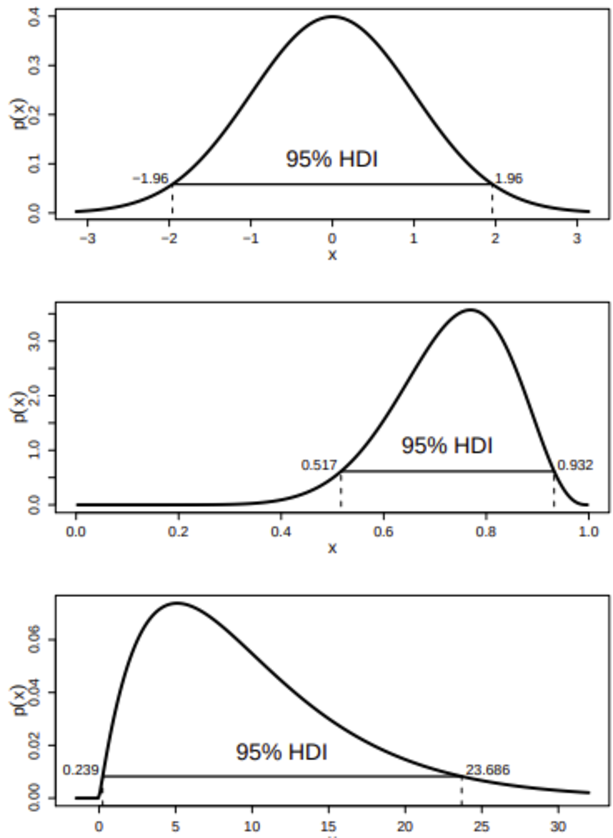
\includegraphics[scale=0.5]{figures/HDI.pdf}
\end{center}
\end{frame}
%%%%%%%%%%%%%%%%%%%%%%%%%%%%%%%%%%%
\begin{frame}{Recommended reading}
\begin{itemize}
  \item[\faBook] \cite{Robert2007}, Ch. 5.
%  \item 
 \item[\faForward] Next lecture: \cite{Robert2007} Ch. 7.
 \end{itemize} 
\end{frame}

%%%%%%%%%%%%%%%%%%%%%%%%%%%%%%%%%%%
\section*{Bayesian model choice}
\begin{frame}{Bayesian model selection: testing all over again}
 Model choice (or selection) is a \textbf{major} topic within any school of inference: it is how scientists make decisions about competing theories/hypotheses in light of data.
 One can associate a set of models $\boldsymbol{\mathcal{M}} = \{ \mathcal{M}_1, \ldots \mathcal{M}_n \}$ with a set of indices $I$ such that $\mu \in I$ we want to estimate the posterior distribution of the indicator function $\mathbb{I}_{\boldsymbol{\Theta}_\mu}(\theta)$.
 
 Recall that estimating indicator functions over $\boldsymbol{\Theta}$ was the fundamental mechanic of Bayesian testing.
 In the setting of Bayesian model selection (BMS), we have something of the form
 \begin{equation*}
  \mathcal{M}_i : x \sim f_i(x \mid \theta_i), \theta_i \in \boldsymbol{\Theta}_i, i \in I.
 \end{equation*}
\end{frame}
%%%%%%%%%%%%%%%%%%%%%%%%%%%%%%%%%%%
\begin{frame}{M-completeness}
A key step in model selection is to identify in which regime the analyst finds themselves in.
\begin{defn}[M-open, M-closed, M-complete]
 \label{def:m-open}
 Model selection can be categorised in three settings:
 \begin{itemize}
  \item \textbf{M-closed}: a situation where the true data-generating model is one of $\mathcal{M}_i \in \boldsymbol{\mathcal{M}}$, even though  it is most often  unknown to the  analyst;
  \item \textbf{M-complete}: a situation where the true model exists and is out of the model set $\boldsymbol{\mathcal{M}}$.
  We nevertheless want to select one of the models in the set due to computational or mathematical tractability reasons.
  \item \textbf{M-open}: a situation in which we know the true data-generating model is not in $\boldsymbol{\mathcal{M}}$ and we have no idea what it looks like.
 \end{itemize}
\end{defn}
See~\cite{Bernardo2000} and \cite{Yao2018}.
\end{frame}
%%%%%%%%%%%%%%%%%%%%%%%%%%%%%%%%%%%
\begin{frame}{BMS: example I}
Suppose one has $x \in \mathbb{N}\cup \{0\}$, which measures, say, the number of eggs Balerion The Black Dread has laid in five consecutive breeding seasons.
One can conjure up
\begin{equation*}
 \mathcal{M}_1 : x \sim \operatorname{Poisson}(\lambda), \lambda > 0,
\end{equation*}
or, if feeling fancy, 
\begin{equation*}
 \mathcal{M}_2 : x \sim \operatorname{Negative-binomial}(\lambda, \phi), \lambda, \phi > 0.
\end{equation*}
Notice that, under $\mathcal{M}_2$, $E[X] = \lambda$ and $\vr(X) = \lambda ( 1 + \lambda/\phi)$.
What happens as $\phi \to \infty$?
\end{frame}
%%%%%%%%%%%%%%%%%%%%%%%%%%%%%%%%%%%
\begin{frame}{BMS: example II}
Take the famous Galaxy data set:
 \begin{center}
 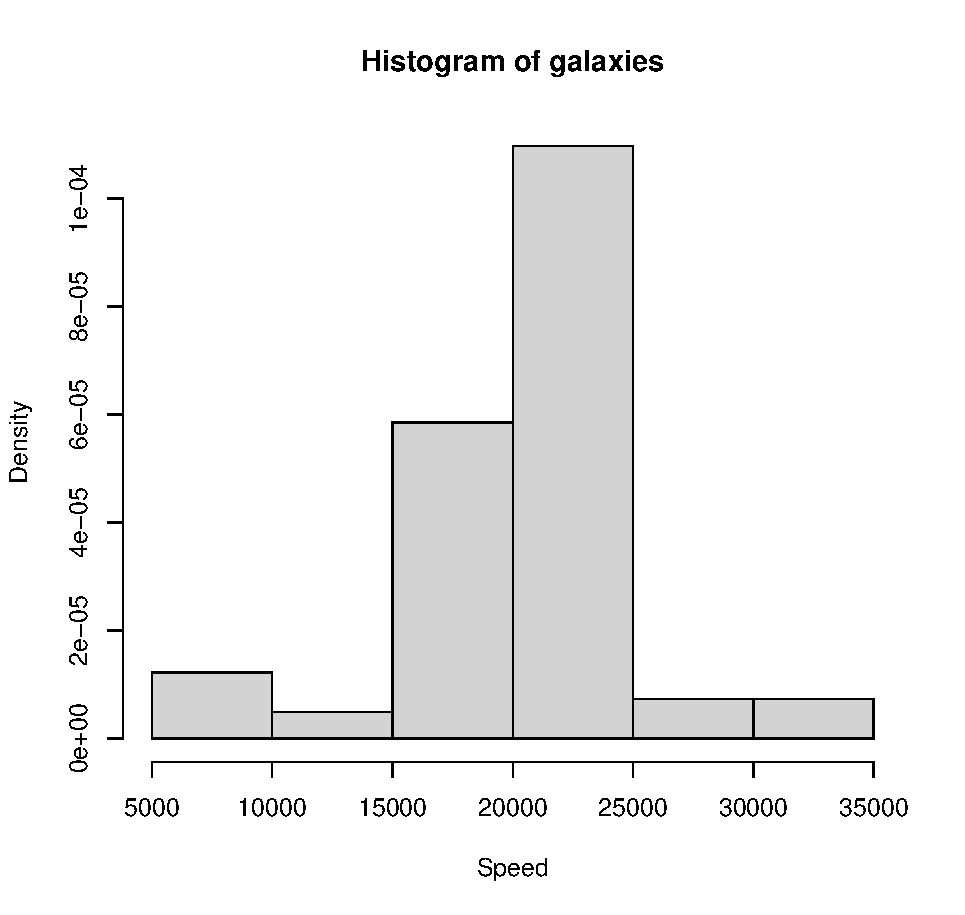
\includegraphics[scale=0.3]{figures/galaxies.pdf}
\end{center}
A now classical model is a Gaussian mixture:
\begin{equation*}
 \mathcal{M}_i : v_j \sim \sum_{l=1}^i p_{il} \cdot \operatorname{Normal}(v_j; \mu_{li},\sigma^2_{li}). 
\end{equation*}
\end{frame}
%%%%%%%%%%%%%%%%%%%%%%%%%%%%%%%%%%%
\begin{frame}{BMS: example III}
Consider the data:
 \begin{center}
 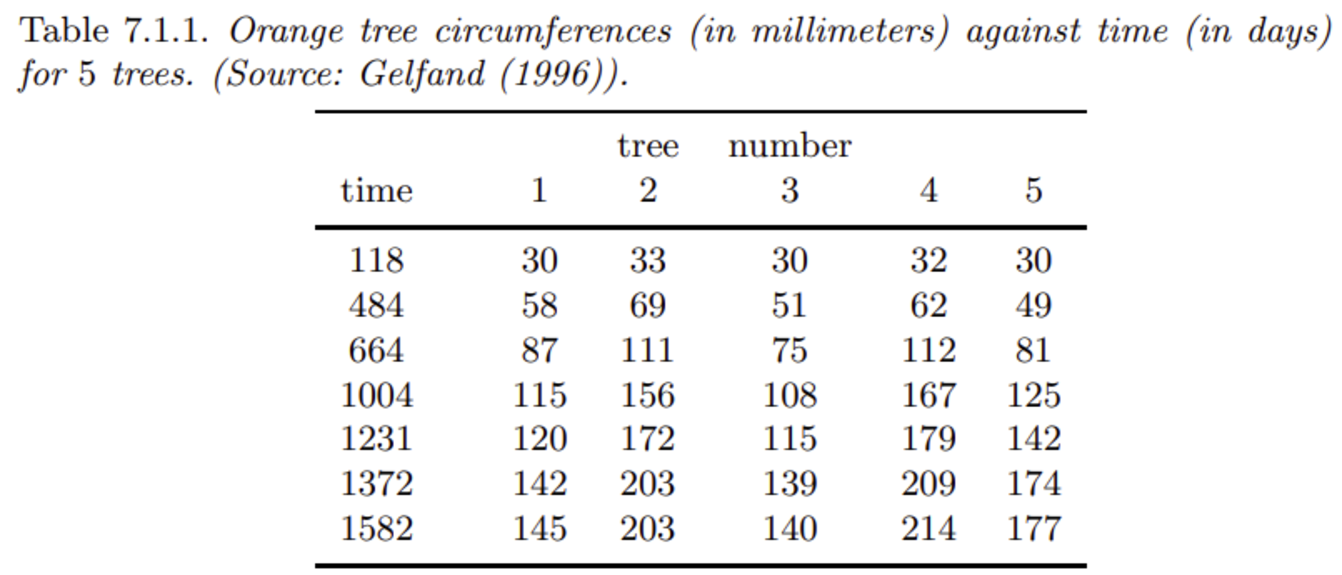
\includegraphics[scale=0.3]{figures/oranges.pdf}
\end{center}
Amongst the models we can consider, 
\begin{align*}
\mathcal{M}_1 :& y_{it} \sim \operatorname{Normal}(\beta_{10} + b_{1i}, \sigma_1^2), \\
\mathcal{M}_2 :& y_{it} \sim \operatorname{Normal}(\beta_{20} + \beta_{21}T_t + b_{2i}, \sigma_2^2) , \\
\mathcal{M}_3 :& y_{it} \sim \operatorname{Normal}\left(\frac{\beta_{30}}{1 + \beta_{31}\exp\left(\beta_{32} T_t\right)}, \sigma_3^2\right), \\
\mathcal{M}_4 :& y_{it} \sim \operatorname{Normal}\left(\frac{\beta_{40} + b_{4i}}{1 + \beta_{41}\exp\left(\beta_{42} T_t\right)}, \sigma_4^2\right).
\end{align*}
\end{frame}
%%%%%%%%%%%%%%%%%%%%%%%%%%%%%%%%%%%
\begin{frame}{Step 0: priors}
First, let us look at a convenient representation of model space:
\begin{equation*}
 \boldsymbol{\Theta} = \bigcup_{i \in I} \{i\} \times \boldsymbol{\Theta}_i.
\end{equation*}
Now, to each $\mathcal{M}_i$, we associate a prior $\pi_i(\theta_i)$  on each subspace and, by Bayes' theorem we get
\begin{align*}
 \pr(\mathcal{M}_i \mid x) & = \pr( \mu = i \mid x), \\ 
 &= \frac{w_i \int_{\boldsymbol{\Theta}_i} f_i(x\mid t_i)\pi_i(t_i)\,dt_i}{\sum_{j} w_j \int_{\boldsymbol{\Theta}_j} f_j(x\mid t_j)\pi_j(t_j)\,dt_j },
\end{align*}
where the $w_i$ are the \textbf{prior probabilities} for each model.
\end{frame}
%%%%%%%%%%%%%%%%%%%%%%%%%%%%%%%%%%%
\begin{frame}{An intuitive predictive}
A nice consequence of the formulation we just saw is that the predictive distribution looks quite intuitive:
\begin{align}
\nonumber
 p(\tilde{x} \mid \boldsymbol{x}) &= \sum_{j} w_j \int_{\boldsymbol{\Theta}_j} f_j(\tilde{x} \mid t_j) f_j(\boldsymbol{x}\mid t_j)\pi_j(t_j)\,dt_j,\\
 \label{eq:predictive_1}
 &= \sum_{j} \pr(\mathcal{M}_j \mid \boldsymbol{x}) m_j(\tilde{x}).
\end{align}
\end{frame}
%%%%%%%%%%%%%%%%%%%%%%%%%%%%%%%%%%%
\begin{frame}{Hello, my old friend}
Here, Bayes factors also play a central role:
\begin{align*}
 \operatorname{BF}_{12} &= \frac{\pr(\mathcal{M}_1 \mid x)}{\pr(\mathcal{M}_2 \mid x)}\bigg/\frac{\pr(\mathcal{M}_1)}{\pr(\mathcal{M}_2)},\\
  &= \frac{w_1^\prime \cdot w_2}{w_2^\prime \cdot w_1},
\end{align*}
with $w_i^\prime := \pr(\mathcal{M}_1 \mid x)$.
\end{frame}
%%%%%%%%%%%%%%%%%%%%%%%%%%%%%%%%%%%
\begin{frame}{Model averaging}
What if we simply \textbf{refuse} to select one model?
We can write
\begin{align}
 \nonumber
 p(\tilde{x} \mid \boldsymbol{x})  &= \int_{\boldsymbol{\Theta}} f(\tilde{x} \mid t) f(\boldsymbol{x}\mid t)\pi(t)\,dt,\\
 \nonumber
 &= \sum_{j} \int_{\boldsymbol{\Theta}_j} f_j(\tilde{x} \mid t_j) g(j, t_j \mid \boldsymbol{x})\,dt_j,\\
 \nonumber
 &= \sum_j p (\mathcal{M}_j \mid \boldsymbol{x}) \int_{\boldsymbol{\Theta}_j} f_j(\tilde{x} \mid t_j) p(t_j \mid \boldsymbol{x})\,dt_j,\\
 \label{eq:predictive_2}
  &= \sum_j w_j^\prime \int_{\boldsymbol{\Theta}_j} f_j(\tilde{x} \mid t_j) p(t_j \mid \boldsymbol{x})\,dt_j.
\end{align}
which is another version of the expression in (\ref{eq:predictive_1}).
\end{frame}
%%%%%%%%%%%%%%%%%%%%%%%%%%%%%%%%%%%
\begin{frame}{Model checking}
Modern Bayesian inference not only allows for, but actively encourages model interrogation and checking.
\begin{itemize}
 \item The central idea of \textbf{Leave-one-out cross-validation (LOO)} is to estimate the \textit{expected log pointwise predictive density for a new dataset}, elpd:
 \begin{equation*}
  \operatorname{elpd} = \sum_{i=1}^n \int m(\tilde{x}_i)\log p(\tilde{x}_i \mid \boldsymbol{x}),d\tilde{x}_i.
 \end{equation*}
 See \cite{Vehtari2017}.
 \item With \textbf{Posterior predictive checks (PPCs)} we wish to compare  functions of the observed data, $f(\boldsymbol{x})$ with functions of the predictive distribution, $f(\boldsymbol{\tilde{x}})$.
  \begin{center}
 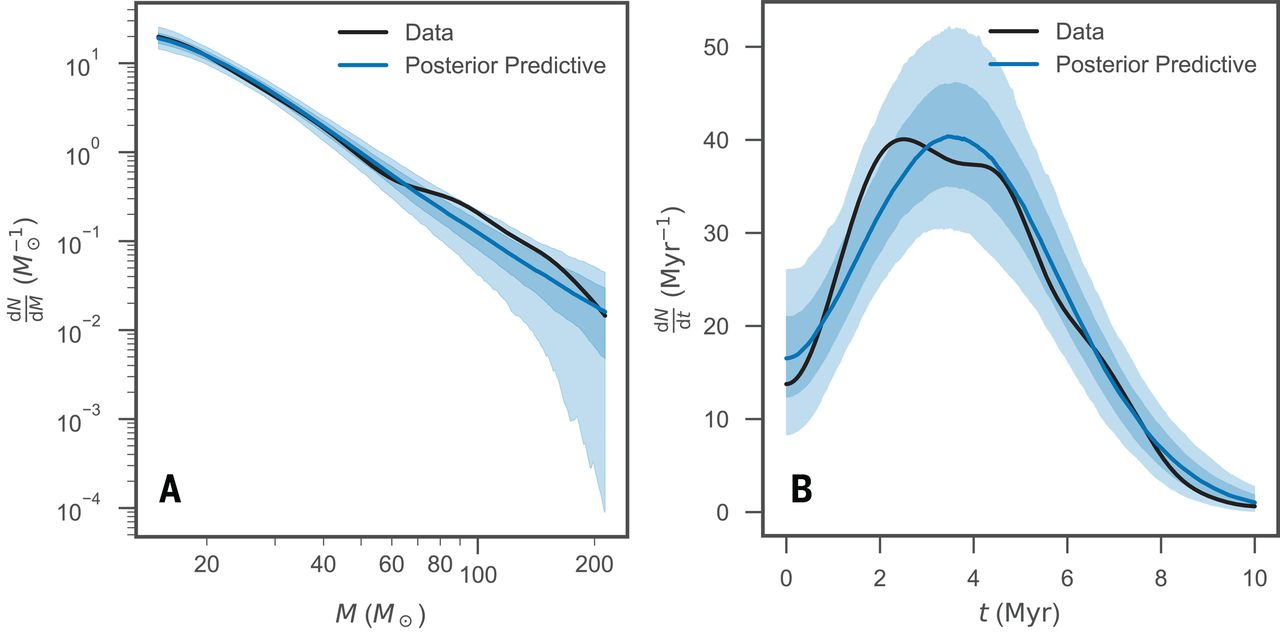
\includegraphics[scale=0.5]{figures/PPC.jpg}
\end{center}
 See \cite{Berkhof2000} and~\cite{Gabry2019}.
\end{itemize}
\end{frame}
%%%%%%%%%%%%%%%%%%%%%%%%%%%%%%%%%%%
\begin{frame}{Recommended reading}
\begin{itemize}
  \item[\faBook] \cite{Robert2007}, Ch. 7.
%  \item 
 \item[\faForward] Next lecture: \cite{Schervish1995} Ch. 7.4.
 \end{itemize} 
\end{frame}

\section*{Bayesian asymptotics}
\begin{frame}{Asymptotics}
A major part of a statistical approach is understanding what happens in the limit of many many observations.
Consider the joint conditional density of the data, $f_n(\boldsymbol{x} \mid \theta)$ and a prior $\pi(\theta)$.
What happens to $p_n(\theta \mid \boldsymbol{x}) = f_n(\boldsymbol{x} \mid \theta)\pi(\theta)/m_n(\boldsymbol{x})$ as $n \to \infty$ ?
\begin{idea}[Asymptotics is about understanding]
 Infinity is a big ``number''.
 Considering what happens  as $n \to \infty$ is less a statement about a real world situation than about the structure and regularity of a model.
 Doing asymptotics is about understanding what makes a model tick rather than getting useful results for a regime seldom achieved in practice.
\end{idea}
Another important aspect to consider is the \textbf{rate} at which things converge asymptotically.
Studying rates provides complementary information about the structure of the model and gives hints as to the accuracy of asymptotic approximations.
 \end{frame}
%%%%%%%%%%%%%%%%%%%%%%%%%%%%%%%%%%%
\begin{frame}{Bayesian asymptotics I: consistency}
\begin{theo}[The posterior concentrates around the ``true'' value]
Let $(S, \mathcal{A}, \mu)$ be a probability space and let $(\Omega, \tau)$ be a finite-dimensional parameter space equipped with a Borel $\sigma$-field.
Suppose there exist measurable $h_n: \mathcal{X}^n \to \Omega$ such that $h_n(\boldsymbol{X})$ converges in probability to $\Theta$.
Writing $\mu_{\boldsymbol{\Theta} \mid \boldsymbol{X}}(\cdot \mid \boldsymbol{x})$ for the posterior measure, we have
\begin{equation*}
 \lim_{n \to \infty} \mu_{\boldsymbol{\Theta} \mid \boldsymbol{X}}(A \mid \boldsymbol{X}) = I_A(\Theta), \: \mu-\textrm{a.s.}
\end{equation*}
\end{theo}
\textbf{Please} see Theorem 7.78 in \cite{Schervish1995} (pg 429) for all of the \textit{many} details.

\textbf{Discussion:} what we are essentially saying here is that if there exists a consistent (sequence of) estimator(s) for $\theta$, then the posterior will concentrate around the true generating distribution of the parameter asymptotically.
\end{frame}
%%%%%%%%%%%%%%%%%%%%%%%%%%%%%%%%%%%
\begin{frame}{Remember Cromwell's law?}
Here is another neat little theorem with a cumbersome proof.
\begin{theo}[A ``nice'' prior ensures posterior consistency]
Define $\operatorname{KL}(\theta, \theta^\prime)$ as the Kullback-Leibler divergence between $P_{\theta}$ and $P_{\theta^\prime}$.
Let $\theta_0$ be the true data-generating parameter and define $C_\epsilon = \{\theta : \operatorname{KL}(\theta_0, \theta) < \epsilon\}$, $\epsilon > 0$.
 Let $\Pi$ be a prior measure such that $\Pi(C_\epsilon) > 0$ for every $\epsilon > 0$.
 Take $N_0$ open such that $C_\epsilon \subset N_0$.
 Then 
 \begin{equation*}
  \lim_{n \to \infty} \mu_{\boldsymbol{\Theta} \mid \boldsymbol{X}}(N_0 \mid \boldsymbol{X}) = 1, \: P_{\theta_0}-\textrm{a.s.}
 \end{equation*}
\end{theo}
Again, \textbf{please} see Theorem 7.80 in \cite{Schervish1995} (pg 430) for the details.
\end{frame}
%%%%%%%%%%%%%%%%%%%%%%%%%%%%%%%%%%%
\begin{frame}[allowframebreaks]{Interlude: regularity conditions}
Before we proceed, we will need to make things nice.
Consider the following regularity conditions
\begin{itemize}
 \item[1] The parameter space is $\boldsymbol{\Theta} \subset \mathbb{R}^d$ for some finite $d$;
 \item[2] We have $\theta_0$ an an interior point of $\boldsymbol{\Theta}$;
 \item[3] The prior distribution has a density w.r.t. Lebesgue which is positive and continuous at $\theta_0$;
 \item[4] There exists $N_0 \subseteq \boldsymbol{\Theta}$ with $\theta_0 \in N_0$ such that the log-likelihood, $l_n(\theta)$, is twice-differentiable with respect to all coordinates of $\theta$, $P_{\theta}$-a.s.
 \item[5] The largest eigenvalue of the inverse observed Fisher information, $\Sigma_n$, vanishes in probability.
 \item[6] The MLE is consistent;
 \item[7] The Fisher information is a smooth function of $\theta$.
\end{itemize}

\end{frame}
%%%%%%%%%%%%%%%%%%%%%%%%%%%%%%%%%%%
\begin{frame}{Bayesian asymptotics II: asymptotic normality}
We can now state a nice result which characterises the asymptotic form of the posterior.
\begin{theo}[Bernstein von-Mises\footnote{Named after Austrian mathematician Richard Edler von Mises (1883--1953) and Russian mathematician Sergei Natanovich Bernstein (1880--1968).}]
Under the regularity conditions we have discussed, take $\hat{\theta}$ to be the MLE.
Put $\boldsymbol{\Psi}_n = \left(\Sigma_n\right)^{-1/2}(\theta- \hat{\theta})$.
Then the posterior distribution of $\boldsymbol{\Psi}_n$ conditional on $\boldsymbol{X}$ converges in probability \textbf{uniformly} on compact sets to the multivariate normal distribution $\operatorname{Normal}_d\left(\boldsymbol{0}, \boldsymbol{I}_d\right)$ with density $\phi_d$.
More precisely,
\begin{equation*}
  \lim_{n \to \infty} P_{\theta_0}\left(\sup_{\psi \in B} \bigg\rvert f_{\boldsymbol{\Psi}_n \mid \boldsymbol{X}}(\psi) - \phi_d(\psi)  \bigg\lvert > \epsilon \right) = 0,
\end{equation*}
for all $B \subset \mathbb{R}^d$ compact and $\epsilon > 0$.
\end{theo}
See Theorem 7.89 in \cite{Schervish1995} (page 437).
\end{frame}
%%%%%%%%%%%%%%%%%%%%%%%%%%%%%%%%%%%
\begin{frame}{Dabbling with normal approximations}
\begin{exercise}[Cauchy location posterior]
 Take $X_i \sim \operatorname{Cauchy}(\theta, 1)$, $i = 1, 2,\ldots, 10$.
 In particular, suppose $\boldsymbol{x} = \{-5, -3, 0, 2, 4, 5, 7, 9, 11, 14\}$.
 \begin{itemize}
  \item[i)] Compute the MLE and $l^{\prime\prime}$;
  \item[ii)] Deduce the parameters of the normal approximation to $p(\theta \mid \boldsymbol{x})$;
  \item[iii)] Use an MCMC\footnote{The instructor can assist with this step.} routine to sample from $p(\theta \mid \boldsymbol{x})$, obtain a posterior approximation to its density and compare it to the normal approximation;
  \item[iv)] Simulate data sets of sizes $n=20, 50, 100, 500, 1000$ and $10, 000$ and repeat iii.
  \item[v)] See if you can reduce/increase the discrepancy between the posterior and its approximation by fiddling with the prior (without breaking the regularity assumptions!).
 \end{itemize}
\end{exercise}
See example 7.104 in \cite{Schervish1995} (page 444).
 \end{frame}
%%%%%%%%%%%%%%%%%%%%%%%%%%%%%%%%%%%
\begin{frame}{Recommended reading}
\begin{itemize}
  \item[\faBook] \cite{Schervish1995} Ch. 7.4.
%  \item 
 \item[\faForward] Next lecture: \cite{Raftery1988} and~\cite{Gelman2002}.
 \end{itemize} 
\end{frame}

%%%%%%%%%%%%%%%%%%%%%%%%%%%%%%%%%%%
\section*{Markov chain Monte Carlo}
\begin{frame}{MCMC: The best bad method you have ever seen}
Markov chain Monte Carlo (MCMC) methods are a broad class of stochastic algorithms to compute integrals.

Suppose you are confronted with the following question: what is the ratio between the circumference of inscribed circle and its diameter?
You are \textbf{not} allowed to use any Geometry.
\begin{figure}
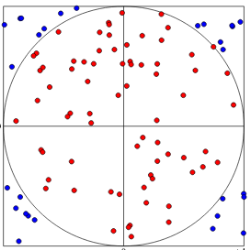
\includegraphics[scale=0.85]{figures/pi_MC.png}
\end{figure}
\end{frame}
%%%%%%%%%%%%%%%%%%%%%%%%%%%%%%%%%%%
\begin{frame}{First, a warning}
\begin{quote}
 ``Monte Carlo is an extremely bad method; it should be used only when all alternative methods are worse.''
\end{quote}
Alan Sokal (1955-) in \textit{Monte Carlo Methods in Statistical Mechanics: Foundations and New Algorithms} (1996, pg. 1).
\begin{figure}
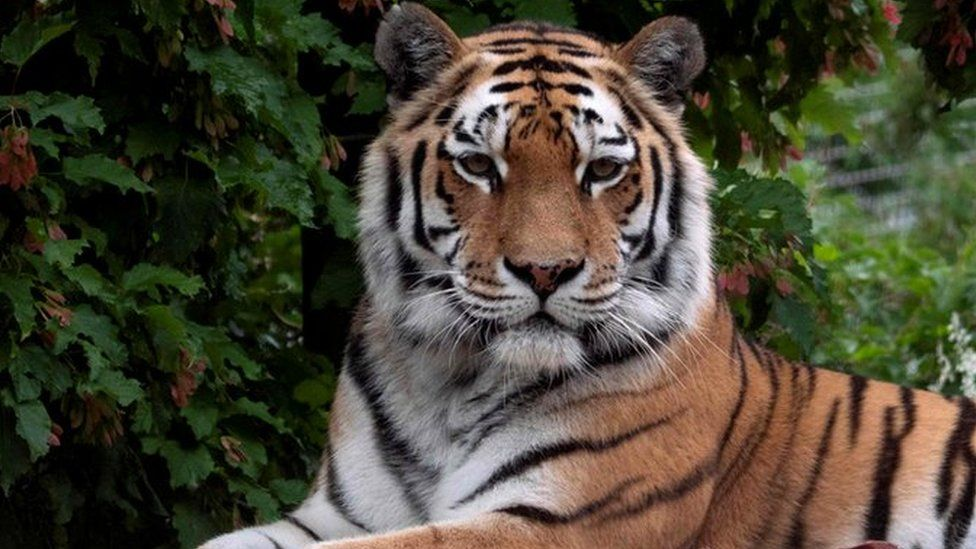
\includegraphics[scale=0.25]{figures/tiger.jpg}
\caption{MCMC is, in a way, like a captive tiger...}
\end{figure}
\end{frame}
%%%%%%%%%%%%%%%%%%%%%%%%%%%%%%%%%%%
\begin{frame}{Also...}
 Repeat after me,
 \begin{idea}[Bayesian MCMC is not a thing]
 \begin{center}
  {\Huge There is no such thing as ``Bayesian'' MCMC.}
 \end{center}  
  
  MCMC is a numerical method for computing integrals.
  It does not care whether you are a Bayesian, frequentist, \textit{flamenguista} or \textit{corintiana}.
 \end{idea}
\end{frame}
%%%%%%%%%%%%%%%%%%%%%%%%%%%%%%%%%%%
\begin{frame}{Computing integrals}
Technically, for a probability space $(X, \mathcal{F}, P)$, for $f : X \to \mathbb{R}$, we want to compute
$$
\mu_f = E_P[f] = \int_{X} f\,dP.  
$$
When $P$ is absolutely continuous with respect to the Lebesgue measure, we have 
$$
\mu_f= \int_{X} f(x)p(x)\,dx,
$$
as is usually written in introductory textbooks.

A ``natural'' approach to obtain an estimator of  $\mu_f$ is
$$
\hat{\mu}_{f, N}^{\text{MC}} = \frac{1}{N} \sum_{n = 1}^{N} f(x_{n}),
$$
with $x_1, \ldots, x_N \sim P$.
\end{frame}
%%%%%%%%%%%%%%%%%%%%%%%%%%%%%%%%%%%
\begin{frame}{A central (limit) theorem}
Define
$$
\text{MC-SE}_{N}[f]
= \sqrt{ \frac{ \text{Var}_{P}[f]}{N} }.
$$
Then
$$
\lim_{N \rightarrow \infty}
\frac{ \hat{\mu}_{f,N}^{\text{MC}} - \mathbb{E}_{P}[f] }
{ \text{MC-SE}_{N}[f] }
\sim \text{Normal}(0, 1),
$$
\begin{idea}[MCMC-CLT needs to hold]
 A key insight is that MCMC only trustworthy when a central limit theorem holds.
 This means $f$ needs to be $2+\epsilon$-integrable with respect to $P$.
 Look out for $\text{MC-SE}$, too. 
 It is important to quantify ``the probable error of the mean''\footnote{A ``pun'' with William Gosset's (1876--1937) paper: Student. (1908). The probable error of a mean. Biometrika, 1-25.}, as it were.
\end{idea}
\end{frame}
%%%%%%%%%%%%%%%%%%%%%%%%%%%%%%%%%%%
\begin{frame}{Diagnostics}
\begin{idea}[Diagnose your MCMC!]
Perhaps as important as learning how to run an MCMC is to learn to \textbf{diagnose} it.
This means detecting failure to converge to $P$ and/or poor statistical performance.
\end{idea}
When running $K$ chains,  the between sample variance can be written as
\begin{equation*}
\label{eq:Between}
 B = \frac{N}{K-1} \sum_{k = 1}^K \left(\bar{x}_k - \bar{\bar{x}}\right)^2, 
\end{equation*}
where $\bar{x}_k = N^{-1}\sum_{n = 1}^N x_k^{(n)}$ and $\bar{\bar{x}} = K^{-1}\sum_{k=1}^K\bar{x}_k$.
Now we can define the within variance as 
\begin{equation*}
W =  K^{-1}\sum_{k = 1}^K s_k^2 \: \text{and} \: s_k^2  = (N-1)^{-1} \sum_{n = 1}^N \left(x_k^{(n)} - \bar{x}_k\right)^2 
\end{equation*}
Finally we can define the~\textbf{potential scale reduction factor} (PSRF)~\citep{Gelman1992}:
\begin{equation*}
 \label{eq:PRSF}
 \hat{R} = \sqrt{\frac{ (N-1)W +  B }{NW}}.
\end{equation*}
At convergence, $\hat{R} < 1.1$, providing a univariate measure of convergence across chains (for a given parameter).
\end{frame}
%%%%%%%%%%%%%%%%%%%%%%%%%%%%%%%%%%%
\begin{frame}{More diagnostics}
One of the things we are interested in is \textit{statistical} performance, i.e., how precise the estimator $\hat{\mu}_{f,N}^{\text{MC}}$ is.
To measure that, we can compute the \textbf{effective sample size}:
\begin{equation*}
 \text{ESS} = \frac{N}{1 + 2\sum_{t=1}^\infty \rho_t},
\end{equation*}
where $\rho_t$ is the \textbf{autocorrelation} at lag $t$, $t=1, 2, \ldots$.
A good rule of thumb\footnote{Assuming approximate normality. Calculation stolen from~\url{https://www.biorxiv.org/content/10.1101/2021.05.04.442586v1.full.pdf}} is that if one wants to have a an standard error which is 1\% of the width of the 95\% interval of the true distribution is to have $\text{ESS} \geq 625$:
\begin{align*}
 \frac{\sigma}{\sqrt{N}} &\leq \frac{\sigma}{\sqrt{\text{ESS}}},\\
 0.01 \times 4 \times \sigma &\leq \frac{\sigma}{\sqrt{\text{ESS}}},\\
 &\implies\\
 \text{ESS} &\geq 625,
\end{align*}
where $\sigma = \sqrt{\text{Var}_{P}[f]}$.
\end{frame}
%%%%%%%%%%%%%%%%%%%%%%%%%%%%%%%%%%%
\begin{frame}{Even more diagnostics}
\begin{figure}
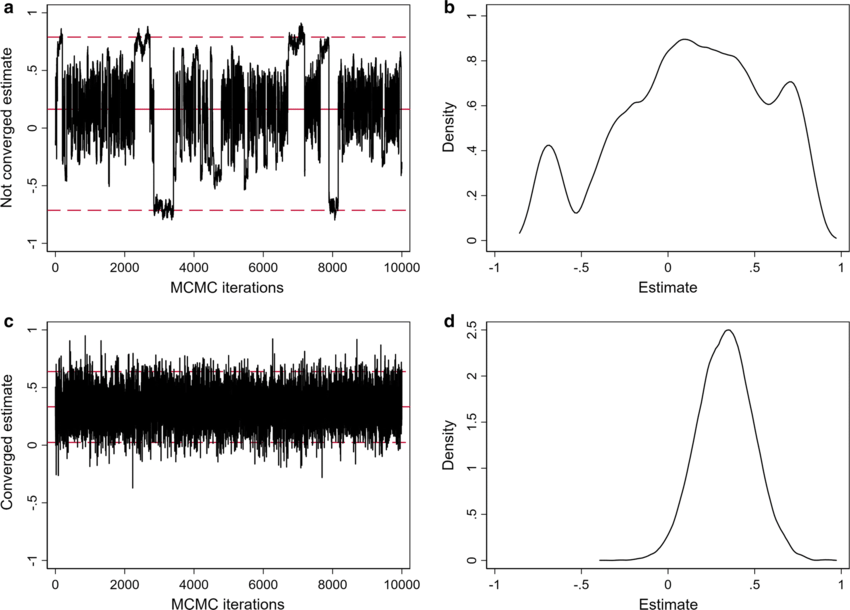
\includegraphics[scale=0.25]{figures/traceplots.png}
\end{figure}
\begin{idea}[No one diagnostic is enough]
 Use multiple diagnostic metrics, always.
 Every MCMC diagnostic out there has blind spots; using multiple simultaneously increases the chances those blind spots are covered.
\end{idea}
\end{frame}
%%%%%%%%%%%%%%%%%%%%%%%%%%%%%%%%%%%
\begin{frame}{Scaling with dimension}
\begin{figure}
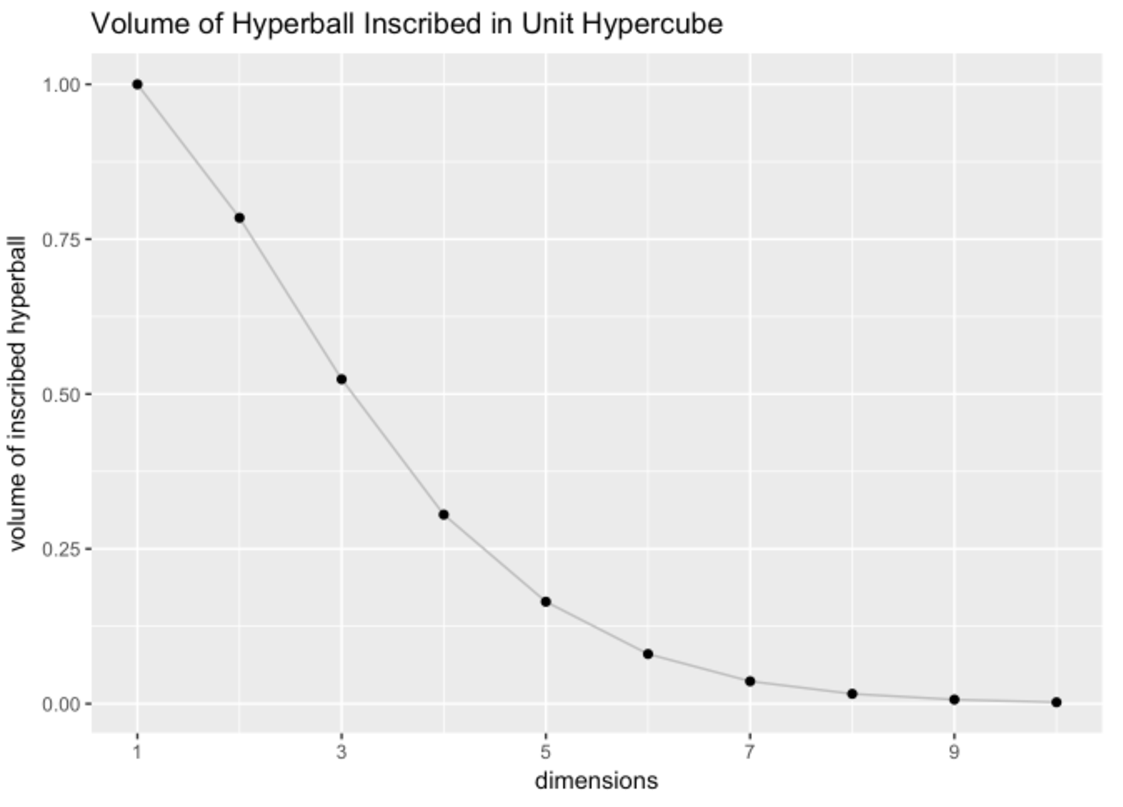
\includegraphics[scale=0.35]{figures/concentration_measure_volume.pdf}
\end{figure}
Taken from~\url{https://mc-stan.org/users/documentation/case-studies/curse-dims.html}.
\begin{idea}[The higher the dimension, the more structure you need]
 As dimension increases, things start to get pretty lonely pretty fast for a particle.
 The only way to counteract this ``thinning'' is to introduce more structure.
 This is the intuitive basis for the success of gradient-based methods such as MALA\footnote{Metropolis-adjusted Langevin algorithm} and HMC\footnote{Hamiltonian (or Hybrid) Monte Carlo.}.
\end{idea}
\end{frame}
%%%%%%%%%%%%%%%%%%%%%%%%%%%%%%%%%%%
\begin{frame}{Take home}
\begin{itemize}
 \item MCMC allows us to make inferences about huge models in Science and Engineering;
 \item MCMC is a terrible method, which nevertheless is our best shot at computing high-dimensional integrals;
 \item One has to make sure a CLT holds;
 \item One has to verify diagnostics to ensure no convergence/performance problems are present;
 \item No one diagnostic is enough.
\end{itemize}
\end{frame}
%%%%%%%%%%%%%%%%%%%%%%%%%%%%%%%%%%%
\begin{frame}{Recommended reading}
\begin{itemize}
  \item[\faBook] \cite{Robert2007}, Ch. 6\footnote{The Bayesian Choice by Christian Robert (2007, 2nd edition).}.
  \item[\faBook] \url{https://betanalpha.github.io/assets/case_studies/markov_chain_monte_carlo.html}
 \end{itemize} 
\end{frame}

%%%%%%%
\begin{frame}[t, allowframebreaks]
\frametitle{References}
\bibliographystyle{apalike}
\bibliography{bayes}
\end{frame}
\end{document}
